\chapter{对偶问题}
\label{chap:duality}

求解约束问题时，算法交出一个可行点，目标值是$0.40625$。这个数够好吗？可行点本身只说明最优值不超过$0.40625$，至于离最优值还差多少，它什么也没有说。第~\ref{chap:constrained-optimality}章的KKT条件能判断一个候选是否满足最优点应有的关系，却不能给一个非最优的候选打分。要回答“还差多少”，必须另有一个不超过最优值的数，也就是下界。

第~\ref{chap:linear-programming}章已经见过这样的下界：把约束乘上权重加起来，得到一份能当场核对的证据。本章把这个办法推广到一般的约束问题。目标和约束不再是线性的，加权之后也就不能靠比较系数得出下界，而要对原变量取一次下确界。

第~\ref{sec:dual-lower-bound}节构造下界，第~\ref{sec:dual-weak}节说明它为什么总是成立，以及怎样用它给可行点估计误差。下确界的计算反复出现“函数加线性项”的结构，第~\ref{sec:dual-conjugate}节把这个结构提取出来，得到计算对偶问题的工具。

最好的下界未必等于最优值。第~\ref{sec:dual-strong}节研究两者何时相等，并把“相等”“原始最优点存在”“最优乘子存在”这三件事分开。第~\ref{sec:dual-certificates}节把上下界、KKT条件和鞍点放到同一对原始—对偶候选上比较，说明它们各自检验了什么。

\section{下界的构造}
\label{sec:dual-lower-bound}

对一般的约束问题，怎样写出一个不依赖未知最优点的下界？全章讨论的问题是
\begin{equation}
 \begin{aligned}
 \min_{\bm{x}\in\bm{D}}\quad & f(\bm{x})\\
 \text{s.t.}\quad & g_i(\bm{x})\leq0,\quad i=1,\ldots,m,\\
 & h_j(\bm{x})=0,\quad j=1,\ldots,p.
 \end{aligned}
 \label{eq:dual-primal}
\end{equation}
这里$\bm{D}\subseteq\mathbb{R}^n$是规定的定义域，$f,g_i,h_j$在其上都取有限值。没有特别说明时$\bm{D}=\mathbb{R}^n$；有些问题只在一部分点上有定义，或者我们有意把一些简单约束（例如$\bm{x}\geq\bm{0}$）留在$\bm{D}$里。

式~\eqref{eq:dual-primal}称为原始问题，它的最优值记为$f^\star$，是可行点上目标值的下确界。没有可行点时规定$f^\star=+\infty$。我们不假设最小点存在，也不假设问题是凸的，这两点在后面都很重要。

第~\ref{chap:constrained-optimality}章为这个问题定义了Lagrange函数，给每条不等式配乘子$\lambda_i$，每条等式配乘子$\nu_j$：
\begin{equation}
 \mathcal{L}(\bm{x},\bm{\lambda},\bm{\nu})=f(\bm{x})+\sum_{i=1}^m\lambda_ig_i(\bm{x})+\sum_{j=1}^p\nu_jh_j(\bm{x}).
 \label{eq:dual-lagrangian}
\end{equation}
那里用它写出候选点上的驻定条件，这里换一个用法：把它当成原目标的一个替身。

\paragraph{用线性价格代替无穷的墙}
约束可以看成目标里的一堵墙。令$\iota_{\leq0}(u)$在$u\leq0$时为$0$，在$u>0$时为$+\infty$，则不等式约束等价于在目标上加$\iota_{\leq0}(g_i(\bm{x}))$。这个函数太硬，无法与目标一起处理。

换成一条斜率$\lambda\geq0$的直线$\lambda u$。图~\ref{fig:dual-wall-price}(a)显示，不论$\lambda$取多少，直线都在墙的下方：$u\leq0$时$\lambda u\leq0$，$u>0$时墙是$+\infty$。用直线替换墙，得到的函数不会超过原来带墙的目标。

这正是价格的想法。约束超支一单位就付$\lambda$的罚款，有结余就按同样的价格退款，违反约束不再被禁止，只是要付钱。等式约束的乘子$\nu_j$没有符号限制，因为$h_j=0$时无论乘什么数，这一项都为零。这个类比只帮助记住不等式的方向，并不表示真的存在这样的市场。

下面用一个能画出来的例子走一遍，全章称它为\emph{一元例}：
\begin{equation}
 \min_{x\in\mathbb{R}}\ \frac12(x-2)^2\quad\text{s.t.}\quad x-1\leq0.
 \label{eq:dual-oned}
\end{equation}
无约束最小点$x=2$不可行，所以解在边界$x^\star=1$上，最优值$f^\star=1/2$。

取$\lambda=1/2$，Lagrange函数是
\[
 \mathcal{L}(x,\tfrac12)=\frac12(x-2)^2+\frac12(x-1).
\]
在可行点$x\leq1$上，第二项不大于零，所以$\mathcal{L}(x,\frac12)\leq f(x)$。图~\ref{fig:dual-wall-price}(b)中，紫色曲线在阴影区都位于蓝色曲线下方，并且全部经过$(1,\frac12)$，因为那里约束的值恰好为零。

对$x$求最小，驻点满足$x-2+\frac12=0$，即$x=\frac32$，最小值是
\[
 \mathcal{L}(\tfrac32,\tfrac12)=\frac18+\frac14=\frac38.
\]
这个最小点并不可行，这没有关系。它是$\mathcal{L}$在整条数轴上的最小值，当然不超过$\mathcal{L}$在可行点上的值，而后者又不超过$f$。于是我们没有用到$x^\star$，就知道$f^\star\geq3/8$。

\begin{BookInlineFigure}
 \centering
 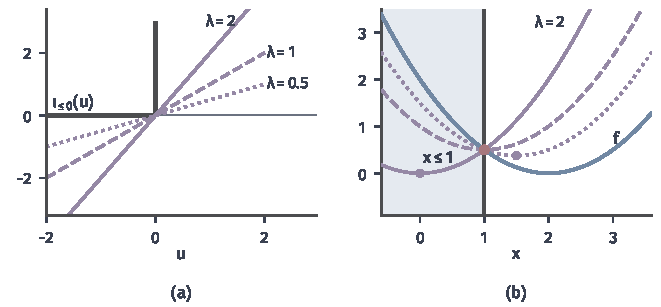
\includegraphics[width=112mm]{figures/05-optimization/06-constrained-optimization/matplotlib/dual-wall-price/figure.pdf}
 \caption{用线性价格代替硬约束。(a)~深灰粗线是硬约束$\iota_{\leq0}(u)$，紫线是$\lambda u$，点线、虚线、实线分别对应$\lambda=0.5,1,2$，都在粗线下方。(b)~一元例~\eqref{eq:dual-oned}：蓝线是目标$f$，浅蓝区域是可行集$x\leq1$，紫线是$\mathcal{L}(\cdot,\lambda)$，线型含义同(a)；紫点是各自的最小点，红点是原始最优点。}
 \label{fig:dual-wall-price}
\end{BookInlineFigure}

这段推理里最容易出错的一步，是必须对$\bm{D}$上的\emph{全部}点取下确界。只求一个驻点是不够的。在$\bm{D}=[-3,3]$上考虑$f(x)=x^3-3x$，约束$x-2\leq0$，取$\lambda=0$，则$\mathcal{L}=f$。驻点$x=1$是局部极小点，值为$-2$，但可行点$x=-3$的目标值是$-18$。局部极小值$-2$不是下界。

\subsection{对偶函数}
\label{sec:dual-function}

把上面的做法写成定义。固定乘子以后，对原变量取下确界，得到的数只依赖乘子。

\begin{definition}[对偶函数]
 \label{def:dual-function}
 问题~\eqref{eq:dual-primal}的\term{对偶函数}（dual function）是
 \begin{equation}
  q(\bm{\lambda},\bm{\nu})=\inf_{\bm{x}\in\bm{D}}\mathcal{L}(\bm{x},\bm{\lambda},\bm{\nu}),
  \label{eq:dual-function}
 \end{equation}
 允许取$-\infty$。使$q$取有限值的乘子组成它的有效定义域$\operatorname{dom}q$。满足$\bm{\lambda}\geq\bm{0}$且$(\bm{\lambda},\bm{\nu})\in\operatorname{dom}q$的乘子称为对偶可行的乘子。
\end{definition}

注意下确界有三种可能，定义中用$\inf$而不是$\min$，正是为了把它们都包括进去。第一种是最小点存在，例如一元例。第二种是下确界为$-\infty$：在$\mathbb{R}$上最小化$-x^2$，约束写成$x-1\leq0$和$-x-1\leq0$，则$\mathcal{L}$对任何乘子都是开口向下的二次函数，$q\equiv-\infty$。这时对偶函数没有提供信息。

第三种是下确界有限但取不到。考虑$\min e^{-x}$，约束$-x\leq0$。取$\lambda=0$，则
\[
 q(0)=\inf_{x\in\mathbb{R}}e^{-x}=0,
\]
这个值没有任何$x$能达到。而$\lambda>0$时，$e^{-x}-\lambda x$在$x\to+\infty$时趋于$-\infty$，所以$q(\lambda)=-\infty$。

现在用第~\ref{chap:constrained-optimality}章的等式二次例计算一个完整的对偶函数，全章称它为\emph{二次例}：
\begin{equation}
 \min_{\bm{x}\in\mathbb{R}^2}\ \frac12(x_1^2+4x_2^2)\quad\text{s.t.}\quad x_1+x_2-1=0.
 \label{eq:dual-quad}
\end{equation}
那里已经由切向导数为零求出最小点$(4/5,1/5)$，最优值是
\[
 f^\star=\frac12\Bigl(\frac{16}{25}+\frac{4}{25}\Bigr)=\frac25.
\]

下面不用这个答案，只用对偶函数。Lagrange函数是
\[
 \mathcal{L}(\bm{x},\nu)=\frac12(x_1^2+4x_2^2)+\nu(x_1+x_2-1).
\]
固定$\nu$，它是$\bm{x}$的严格凸二次函数，令梯度为零就得到唯一的全局最小点：
\[
 x_1+\nu=0,\qquad 4x_2+\nu=0.
\]
因此
\[
 x_1(\nu)=-\nu,\qquad x_2(\nu)=-\frac{\nu}{4}.
\]

代回$\mathcal{L}$，两个平方项和约束项分别是
\[
 \frac12\Bigl(\nu^2+\frac{\nu^2}{4}\Bigr)=\frac58\nu^2,\qquad
 \nu\Bigl(-\nu-\frac{\nu}{4}-1\Bigr)=-\frac54\nu^2-\nu.
\]
相加得到关于$\nu$的一元函数
\begin{equation}
 q(\nu)=-\frac58\nu^2-\nu.
 \label{eq:dual-quad-q}
\end{equation}

这是一条开口向下的抛物线。令导数$-\frac54\nu-1=0$，得到
\[
 \nu^\star=-\frac45,\qquad q(\nu^\star)=-\frac25+\frac45=\frac25.
\]
最好的下界恰好等于$f^\star=2/5$，同时$\bm{x}(\nu^\star)=(4/5,1/5)$也正是原问题的解。

图~\ref{fig:dual-equality-q}(a)显示了这个过程。$\nu$的作用是在目标上加一个倾斜的线性项，把碗底从原点沿紫色虚线推走。$\nu=0$时碗底在原点，不满足约束；$\nu=-4/5$时碗底恰好落到约束直线上。图~\ref{fig:dual-equality-q}(b)是这个过程中碗底的高度随$\nu$的变化，也就是$q(\nu)$。

\begin{BookInlineFigure}
 \centering
 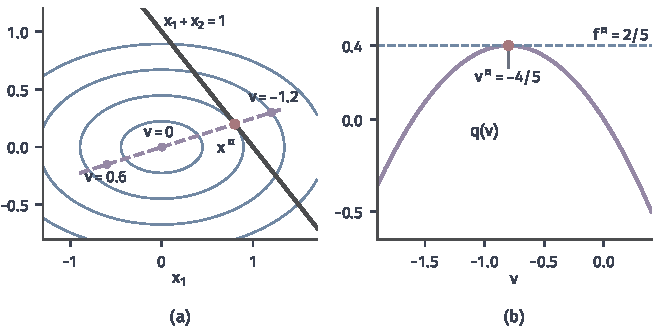
\includegraphics[width=112mm]{figures/05-optimization/06-constrained-optimization/matplotlib/dual-equality-q/figure.pdf}
 \caption{二次例~\eqref{eq:dual-quad}的对偶函数。(a)~蓝线是目标的等高线，深灰粗线是约束$x_1+x_2=1$，紫色虚线是内层最小点$\bm{x}(\nu)=(-\nu,-\nu/4)$的轨迹，红点是$\bm{x}^\star$。(b)~紫线是$q(\nu)$，它处处不超过蓝色虚线$f^\star$，在$\nu^\star=-4/5$处相等。}
 \label{fig:dual-equality-q}
\end{BookInlineFigure}

不等式约束的对偶函数要多处理一件事：内层的$\bm{D}$可以有边界，最小点会在边界上换挡。第~\ref{chap:constrained-optimality}章的预算例取$\tau=2$，就是这种情形，全章称它为\emph{预算例}：
\begin{equation}
 \min_{\bm{x}\geq\bm{0}}\ \frac12\bigl[(x_1-2)^2+(x_2-1)^2\bigr]\quad\text{s.t.}\quad x_1+x_2-2\leq0.
 \label{eq:dual-budget}
\end{equation}
把$\bm{x}\geq\bm{0}$留在$\bm{D}=\mathbb{R}^2_{+}$中，只给预算约束配乘子$\lambda\geq0$。

此时内层问题按坐标分开：
\[
 \min_{x_1\geq0}\Bigl[\frac12(x_1-2)^2+\lambda x_1\Bigr]+\min_{x_2\geq0}\Bigl[\frac12(x_2-1)^2+\lambda x_2\Bigr]-2\lambda.
\]
每一项是开口向上的一元二次函数在半轴上的最小化，最小点是无约束最小点截断到非负：
\[
 x_1(\lambda)=\max\{2-\lambda,0\},\qquad x_2(\lambda)=\max\{1-\lambda,0\}.
\]

$\lambda$越过$1$时第二个坐标碰到边界，越过$2$时第一个坐标也碰到边界。分三段代入，得到
\begin{equation}
 q(\lambda)=\begin{cases}
 \lambda-\lambda^2, & 0\leq\lambda\leq1,\\
 \dfrac12-\dfrac12\lambda^2, & 1\leq\lambda\leq2,\\
 \dfrac52-2\lambda, & \lambda\geq2.
 \end{cases}
 \label{eq:dual-budget-q}
\end{equation}

三段在分界点连续：$\lambda=1$时都是$0$，$\lambda=2$时都是$-3/2$。第一段的最大点是$\lambda^\star=1/2$，最好的下界是$q(1/2)=1/4$。

这个例子的解是$\bm{x}^\star=(3/2,1/2)$，目标值$\frac12(\frac14+\frac14)=\frac14$，下界再次与最优值相等。图~\ref{fig:dual-budget-q}中，内层最小点随$\lambda$增大沿折线向原点移动，价格越高，用得越少；$q$相应地分成三段。

\begin{BookInlineFigure}
 \centering
 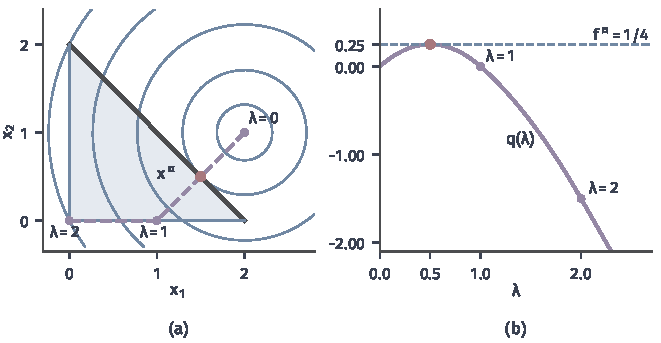
\includegraphics[width=112mm]{figures/05-optimization/06-constrained-optimization/matplotlib/dual-budget-q/figure.pdf}
 \caption{预算例~\eqref{eq:dual-budget}的对偶函数。(a)~浅蓝区域是可行集，深灰粗线是预算约束，蓝线是目标等高线，紫色虚线是内层最小点$\bm{x}(\lambda)$随$\lambda$从$0$增大的轨迹，紫点是$\lambda=0,1,2$时的位置，红点是$\bm{x}^\star$。(b)~紫线是分段的$q(\lambda)$，紫点是分界点，红点是最大点$(1/2,1/4)$。}
 \label{fig:dual-budget-q}
\end{BookInlineFigure}

\subsection{对偶问题}
\label{sec:dual-problem}

每组合法的乘子给出一个下界，下界越大提供的信息越多。很自然地，我们想要最大的那个，于是得到一个新的优化问题。

\begin{definition}[对偶问题]
 \label{def:dual-problem}
 问题~\eqref{eq:dual-primal}的对偶问题是在合法乘子上最大化对偶函数，
 \begin{equation}
  d^\star=\sup_{\bm{\lambda}\geq\bm{0},\ \bm{\nu}}q(\bm{\lambda},\bm{\nu}),
  \label{eq:dual-problem}
 \end{equation}
 其最优值$d^\star$可以取$\pm\infty$；对偶可行的乘子不存在时$d^\star=-\infty$。达到这个上确界的乘子称为对偶最优乘子。
\end{definition}

这里的约束只有$\bm{\lambda}\geq\bm{0}$，比原问题简单。更值得注意的是目标函数的形状。图~\ref{fig:dual-budget-q}(b)和图~\ref{fig:dual-equality-q}(b)中的$q$都是凹的，这不是巧合。

要看出原因，把$\mathcal{L}$反过来读：固定$\bm{x}$，它关于乘子是仿射函数，斜率是约束值$g_i(\bm{x})$与$h_j(\bm{x})$，截距是$f(\bm{x})$。$q$是这一族直线的下包络。图~\ref{fig:dual-affine-envelope}中一元例的每条直线对应一个$x$，它们的下包络（紫线）向下弯曲。

\begin{theorem}[对偶函数是凹的]
 \label{thm:dual-concave}
 对问题~\eqref{eq:dual-primal}，无论$f,g_i,h_j$和$\bm{D}$是否凸，$q$都是凹函数，$\operatorname{dom}q$是凸集。
\end{theorem}

\begin{proof}
 记$\bm{a}=(\bm{\lambda},\bm{\nu})$。任取$\bm{a}_1,\bm{a}_2$和$\theta\in[0,1]$，令$\bm{a}=\theta\bm{a}_1+(1-\theta)\bm{a}_2$。$\mathcal{L}$对乘子是仿射的，所以对每个$\bm{x}\in\bm{D}$，
 \[
  \mathcal{L}(\bm{x},\bm{a})=\theta\mathcal{L}(\bm{x},\bm{a}_1)+(1-\theta)\mathcal{L}(\bm{x},\bm{a}_2).
 \]
 由下确界的定义，右端不小于$\theta q(\bm{a}_1)+(1-\theta)q(\bm{a}_2)$。对$\bm{x}\in\bm{D}$取下确界，得到
 \[
  q(\bm{a})\geq\theta q(\bm{a}_1)+(1-\theta)q(\bm{a}_2).
 \]
 若$\bm{a}_1,\bm{a}_2\in\operatorname{dom}q$，右端有限，于是$\bm{a}\in\operatorname{dom}q$。
\end{proof}

\begin{BookInlineFigure}
 \centering
 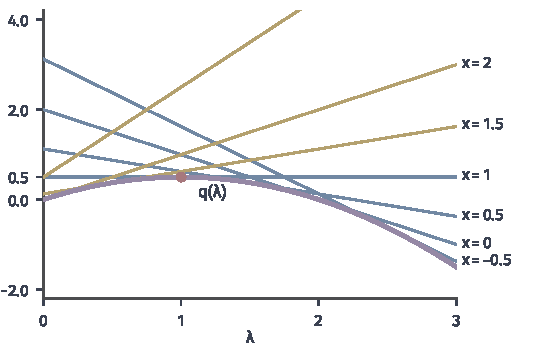
\includegraphics[width=92mm]{figures/05-optimization/06-constrained-optimization/matplotlib/dual-affine-envelope/figure.pdf}
 \caption{一元例中，每个固定的$x$给出一条直线$\lambda\mapsto\mathcal{L}(x,\lambda)$，蓝线对应可行的$x$，黄线对应不可行的$x$（最陡的一条是$x=3$），紫线是下包络$q(\lambda)=\lambda-\lambda^2/2$。可行点的直线斜率不为正，所以在$\lambda\geq0$上不超过其截距$f(x)$；水平粗线是$x=1$，高度为$f^\star=1/2$，在红点处与$q$相切。}
 \label{fig:dual-affine-envelope}
\end{BookInlineFigure}

定理~\ref{thm:dual-concave}说的是一个凸优化问题总摆在手边，无论原问题多么复杂，最大化一个凹函数原则上没有多余的局部最优。但这并不意味着对偶问题容易求解。计算$q$的一个值就要做一次内层的全局最小化，而内层目标$\mathcal{L}(\cdot,\bm{\lambda},\bm{\nu})$可以和原目标一样非凸。前面$f(x)=x^3-3x$的例子说明，局部解在这里给不出下界。凹性属于外层，难度可能全部留在内层。

线性规划是内层可以完全算出的特例。把第~\ref{chap:linear-programming}章的标准型$\min\bm{c}^\top\bm{x}$，$\bm{A}\bm{x}=\bm{b}$，$\bm{x}\geq\bm{0}$放进这个框架，取$\bm{D}=\mathbb{R}^n$。给不等式$-\bm{x}\leq\bm{0}$配乘子$\bm{s}\geq\bm{0}$，给等式配乘子$-\bm{y}$，则
\[
 \mathcal{L}=\bm{c}^\top\bm{x}-\bm{y}^\top(\bm{A}\bm{x}-\bm{b})-\bm{s}^\top\bm{x}=\bm{b}^\top\bm{y}+(\bm{c}-\bm{A}^\top\bm{y}-\bm{s})^\top\bm{x}.
\]

这是$\bm{x}$的线性函数，只有斜率为零时下确界才有限：
\[
 q(\bm{s},\bm{y})=\begin{cases}\bm{b}^\top\bm{y}, & \bm{A}^\top\bm{y}+\bm{s}=\bm{c},\\ -\infty, & \text{其他情形}.\end{cases}
\]
第~\ref{chap:linear-programming}章对偶问题的等式约束$\bm{A}^\top\bm{y}+\bm{s}=\bm{c}$，在这里的含义是$\operatorname{dom}q$的条件。把$q=-\infty$的乘子排除后，再最大化$\bm{b}^\top\bm{y}$，就回到了那里的对偶问题。

\section{弱对偶}
\label{sec:dual-weak}

上一节在例子里反复看到“下界不超过最优值”。这个结论在什么范围内成立，它又能为手里的候选点提供什么？

\begin{theorem}[弱对偶]
 \label{thm:dual-weak}
 对问题~\eqref{eq:dual-primal}的任一可行点$\bm{x}$和任一组$\bm{\lambda}\geq\bm{0}$、$\bm{\nu}$，有
 \begin{equation}
  q(\bm{\lambda},\bm{\nu})\leq f(\bm{x}).
  \label{eq:dual-weak-pair}
 \end{equation}
 因而
 \begin{equation}
  d^\star\leq f^\star.
  \label{eq:dual-weak}
 \end{equation}
\end{theorem}

\begin{proof}
 由可行性和$\bm{\lambda}\geq\bm{0}$，有$\lambda_ig_i(\bm{x})\leq0$和$\nu_jh_j(\bm{x})=0$，所以这些项都不使$f(\bm{x})$增大。又因为$\bm{x}\in\bm{D}$，由下确界的定义，
 \[
  q(\bm{\lambda},\bm{\nu})\leq\mathcal{L}(\bm{x},\bm{\lambda},\bm{\nu})\leq f(\bm{x}).
 \]
 左边不含$\bm{x}$，对可行点取下确界，再对合法乘子取上确界，就得到式~\eqref{eq:dual-weak}。没有可行点时$f^\star=+\infty$，式~\eqref{eq:dual-weak}自然成立。
\end{proof}

证明只用了两件事：下确界的定义，以及符号。它不需要凸性，不需要可微性，也不需要任何约束资格。正因为条件这样少，弱对偶可以用于任何问题，这是它最大的价值。

\term{弱对偶}这个名字在第~\ref{chap:linear-programming}章已经出现过，那里说的是线性规划的特例。两个差要分清。一个是某一对候选的差$f(\bm{x})-q(\bm{\lambda},\bm{\nu})$，下面称为\emph{候选间隙}，算法每一步都能算出。另一个是两个最优值的差$f^\star-d^\star$，这是问题本身的性质，称为\term{对偶间隙}。候选间隙总不小于对偶间隙。

\paragraph{在目标—约束平面上看弱对偶}
把每个$x$映成平面上的一点$(u,t)=(g(x),f(x))$，横坐标是约束值，纵坐标是目标值，这些点组成集合$\bm{G}$。对一元例，$u=x-1$，$t=\frac12(u-1)^2$，$\bm{G}$是一条抛物线，如图~\ref{fig:dual-image-set}所示。可行点对应$u\leq0$，原始问题就是在竖线左侧找$\bm{G}$的最低点。

$\mathcal{L}=t+\lambda u$在斜率为$-\lambda$的直线上为常数。$q(\lambda)$就是把这样的直线从下方推到刚好碰到$\bm{G}$，这条直线与竖轴$u=0$的交点高度。

所以弱对偶的几何含义是：直线在$\bm{G}$下方，$\lambda\geq0$时它在$u\leq0$一侧向左不下降，因此$\bm{G}$中$u\leq0$的部分都在交点上方。对偶问题就是转动直线，使交点尽量高。$\lambda$取负数时直线向左下降，交点就可能高过可行部分的最低点，后面会看到这个现象。

\begin{BookInlineFigure}
 \centering
 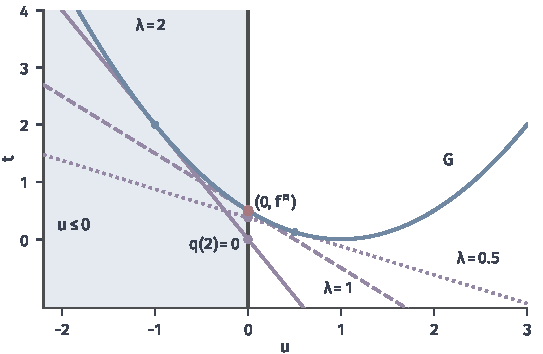
\includegraphics[width=92mm]{figures/05-optimization/06-constrained-optimization/matplotlib/dual-image-set/figure.pdf}
 \caption{一元例在$(u,t)=(g(x),f(x))$平面上的像。蓝线是$\bm{G}$，浅蓝区域是可行的半平面$u\leq0$，深灰粗线是$u=0$。紫线是斜率$-\lambda$的支撑直线（$\lambda=0.5,1,2$，分别为点线、虚线、实线），它们在$\bm{G}$下方，与$u=0$的交点（紫点）高度就是$q(\lambda)$，分别为$0.375$、$0.5$、$0$。红点$(0,f^\star)$是$\lambda=1$时的切点。}
 \label{fig:dual-image-set}
\end{BookInlineFigure}

\subsection{可行候选的误差证书}
\label{sec:dual-certificate}

现在回答本章开头的问题。手里有一个可行点$\hat{\bm{x}}$和一组合法乘子$(\bm{\lambda},\bm{\nu})$，由弱对偶，最优值被夹在两个可计算的数之间：
\begin{equation}
 q(\bm{\lambda},\bm{\nu})\leq f^\star\leq f(\hat{\bm{x}}).
 \label{eq:dual-sandwich}
\end{equation}
两边同时减去，得到次优性的一个可以计算的上界：
\begin{equation}
 0\leq f(\hat{\bm{x}})-f^\star\leq f(\hat{\bm{x}})-q(\bm{\lambda},\bm{\nu}).
 \label{eq:dual-gap-certificate}
\end{equation}
右端不含$f^\star$，这一对候选本身就是一份\emph{误差证书}。第~\ref{chap:optimization}章讨论过目标差难以计算的困难，这里给出了一种解决办法。

用二次例算一组不是最优的候选。取可行点和乘子
\[
 \hat{\bm{x}}=\Bigl(\frac34,\frac14\Bigr),\qquad\nu=-\frac34.
\]
原始目标值由定义计算，对偶目标值由式~\eqref{eq:dual-quad-q}计算：
\[
 f(\hat{\bm{x}})=\frac12\Bigl(\frac{9}{16}+\frac{4}{16}\Bigr)=\frac{13}{32},\qquad
 q\Bigl(-\frac34\Bigr)=-\frac{45}{128}+\frac34=\frac{51}{128}.
\]

候选间隙是
\[
 \frac{13}{32}-\frac{51}{128}=\frac{52-51}{128}=\frac{1}{128}\approx0.0078.
\]
所以不用知道答案，我们就确认$\hat{\bm{x}}$的目标差不超过$0.0078$。

因为这个例子知道答案，可以核对证书有多紧。真实目标差和乘子一侧的差分别是
\[
 \frac{13}{32}-\frac25=\frac{1}{160},\qquad\frac25-\frac{51}{128}=\frac{1}{640}.
\]
两者之和是
\[
 \frac{1}{160}+\frac{1}{640}=\frac{5}{640}=\frac{1}{128},
\]
正是候选间隙。候选间隙同时度量了原始和对偶两侧的误差，图~\ref{fig:dual-certificate-line}把这几个数放在同一条数轴上。

\begin{BookInlineFigure}
 \centering
 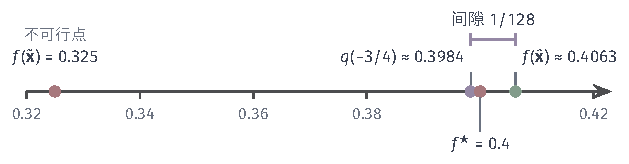
\includegraphics[width=106.4mm]{figures/05-optimization/06-constrained-optimization/tikz/dual-certificate-line/figure.pdf}
 \caption{二次例的误差证书。紫点是下界$q(-3/4)$，绿点是可行点$\hat{\bm{x}}$的目标值，红点$f^\star$夹在两者之间，紫色括线是候选间隙。左边的红点是不可行点$\tilde{\bm{x}}=(0.7,0.2)$的目标值，它比$f^\star$低，不能用来估计误差。}
 \label{fig:dual-certificate-line}
\end{BookInlineFigure}

式~\eqref{eq:dual-gap-certificate}有三个前提，每一个都要单独检验，下面逐一看缺了会怎样。

第一个是原始可行性。点$\tilde{\bm{x}}=(0.7,0.2)$不满足约束，因为$0.7+0.2\neq1$。它的目标值只有
\[
 f(\tilde{\bm{x}})=\frac12(0.49+0.16)=0.325,
\]
比最优值低，与下界的差是$0.325-0.3984\approx-0.073$，是负数。负的“间隙”在这里暴露了不可行，但一般不能指望这样：不可行点也可能给出正的小间隙。所以约束残差要另外计算，不能从间隙看出来。

第二个是乘子的合法性。考虑$\min x^2$，约束$x-1\leq0$，最优值$f^\star=0$。内层最小点是$x=-\lambda/2$，代回得到
\[
 q(\lambda)=-\frac{\lambda^2}{4}-\lambda.
\]
这个公式对负的$\lambda$照样能算，例如$\lambda=-2$时给出$q=1$，比真实最优值$0$还大。

错在哪里？$\lambda=-2$时，可行点$x=0$上的$\mathcal{L}=0-2(0-1)=2$，比$f(0)=0$大，证明中$\mathcal{L}\leq f$这一步失效。图~\ref{fig:dual-illegal-multiplier}中红色虚线高过了$f^\star$，这段就是不合法的乘子。

\begin{BookInlineFigure}
 \centering
 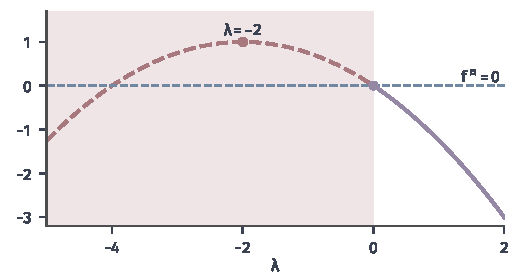
\includegraphics[width=88mm]{figures/05-optimization/06-constrained-optimization/matplotlib/dual-illegal-multiplier/figure.pdf}
 \caption{乘子合法性的作用。问题是$\min x^2$，约束$x-1\leq0$。紫线是$\lambda\geq0$时的$q(\lambda)$，始终不超过蓝色虚线$f^\star=0$；红色虚线和浅红区域对应$\lambda<0$，同一个公式在这里可以超过$f^\star$，例如$\lambda=-2$时为$1$，它不是下界。}
 \label{fig:dual-illegal-multiplier}
\end{BookInlineFigure}

第三个前提是下界本身算得可信，也就是内层下确界确实是下确界。这一点在实际计算中最容易被忽略，单独放在下一小节讨论。

\subsection{内层近似的方向}
\label{sec:dual-inexact-inner}

计算$q$需要解一个最小化问题。多数情况下内层得不到解析解，只能迭代到某个近似点$\tilde{\bm{x}}$。这样算出的$\mathcal{L}(\tilde{\bm{x}},\bm{\lambda},\bm{\nu})$可不可以当作下界使用？

答案是不可以，而且误差的方向恰好不对。由下确界的定义，
\[
 \mathcal{L}(\tilde{\bm{x}},\bm{\lambda},\bm{\nu})\geq q(\bm{\lambda},\bm{\nu}),
\]
近似值落在真正下界的\emph{上方}。普通的数值误差只让答案不够精确，这里的误差却可能让“下界”超过最优值，于是证书本身失效。

还是看二次例，固定$\nu=-3/4$。精确的内层解是$\bm{x}(\nu)=(3/4,3/16)$。假设迭代停在
\[
 \tilde{\bm{x}}=(0.8,0.15).
\]
此处的Lagrange函数值是
\[
 \mathcal{L}(\tilde{\bm{x}},\nu)=\frac12(0.64+0.09)-0.75\,(0.8+0.15-1)=0.365+0.0375=0.4025.
\]
这个数比$f^\star=0.4$还大。如果把它当作下界，就会得出一个错误的结论，以为最优值不小于$0.4025$。

要得到可靠的下界，必须从近似值中扣除一个经过证明的量。若内层函数有已知的曲率下界，用梯度残差就可以写出这个量。

\begin{lemma}[由梯度残差得到的认证下界]
 \label{lem:dual-certified-bound}
 设$\bm{D}=\mathbb{R}^n$，$\bm{\lambda}\geq\bm{0}$，函数$\mathcal{L}(\cdot,\bm{\lambda},\bm{\nu})$可微且是$\mu$强凸的，$\mu>0$。则对任意$\tilde{\bm{x}}$，
 \begin{equation}
  q(\bm{\lambda},\bm{\nu})\geq\mathcal{L}(\tilde{\bm{x}},\bm{\lambda},\bm{\nu})-\frac{1}{2\mu}\bigl\lVert\nabla_{\bm{x}}\mathcal{L}(\tilde{\bm{x}},\bm{\lambda},\bm{\nu})\bigr\rVert_2^2.
  \label{eq:dual-certified-bound}
 \end{equation}
\end{lemma}

\begin{proof}
 记$\phi=\mathcal{L}(\cdot,\bm{\lambda},\bm{\nu})$，$\bm{r}=\nabla\phi(\tilde{\bm{x}})$。由$\mu$强凸的一阶不等式，对任意$\bm{y}$，
 \[
  \phi(\bm{y})\geq\phi(\tilde{\bm{x}})+\langle\bm{r},\bm{y}-\tilde{\bm{x}}\rangle+\frac{\mu}{2}\lVert\bm{y}-\tilde{\bm{x}}\rVert_2^2.
 \]
 右端是$\bm{y}$的二次函数，在$\bm{y}=\tilde{\bm{x}}-\bm{r}/\mu$处最小，最小值为$\phi(\tilde{\bm{x}})-\lVert\bm{r}\rVert_2^2/(2\mu)$。于是对任意$\bm{y}$，
 \[
  \phi(\bm{y})\geq\phi(\tilde{\bm{x}})-\frac{1}{2\mu}\lVert\bm{r}\rVert_2^2.
 \]
 对$\bm{y}$取下确界即得。
\end{proof}

式~\eqref{eq:dual-certified-bound}的含义是：曲率下界$\mu$限制了函数在$\tilde{\bm{x}}$附近能下降多少，碗不会比它更平，所以梯度残差所能带来的下降有上限，我们把这个上限全部扣掉。

代入例子。Hessian是$\operatorname{diag}(1,4)$，取$\mu=1$。梯度和扣除量分别是
\[
 \nabla_{\bm{x}}\mathcal{L}(\tilde{\bm{x}},\nu)=(x_1+\nu,\,4x_2+\nu)=(0.05,-0.15),\qquad\frac{1}{2\mu}\lVert\cdot\rVert_2^2=\frac{0.025}{2}=0.0125.
\]
认证下界是
\[
 0.4025-0.0125=0.39.
\]

它确实低于真正的$q(-3/4)=0.3984$。图~\ref{fig:dual-inner-approx}把这些数排在一起：未修正的内层值在$f^\star$上方，认证下界在$q$下方。把它和$f(\hat{\bm{x}})=0.40625$配对，得到的候选间隙是$0.01625$，比精确内层的$0.0078$宽，但它是可信的。

\begin{BookInlineFigure}
 \centering
 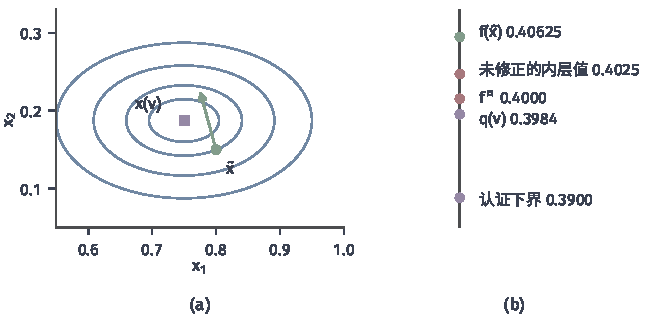
\includegraphics[width=112mm]{figures/05-optimization/06-constrained-optimization/matplotlib/dual-inner-approx/figure.pdf}
 \caption{近似内层的方向。(a)~蓝线是$\mathcal{L}(\cdot,-3/4)$的等高线，紫色方块是精确内层解$\bm{x}(\nu)$，绿点是近似点$\tilde{\bm{x}}$，绿色箭头是负梯度方向。(b)~数轴上由下往上是认证下界、精确的$q(\nu)$、$f^\star$、未修正的内层值和可行点的目标值；未修正的内层值高于$f^\star$，不能当作下界。}
 \label{fig:dual-inner-approx}
\end{BookInlineFigure}

式中的$\mu$必须是真正的曲率下界。若误把$\mathcal{L}$的最大曲率$4$当作$\mu$，扣除量只有$0.025/8=0.003125$，得到$0.399375$，已经超过真正的$q=0.3984$，证书不再成立。当内层没有已知的强凸常数，或者$\bm{D}$不是全空间时，这个引理不能直接使用；此时内层的近似值只能算是一个估计，不能写进误差证书。

\section{凸共轭}
\label{sec:dual-conjugate}

计算对偶函数时，内层总是“目标加上一个线性项，再取下确界”。线性等式约束$\bm{A}\bm{x}=\bm{b}$的对偶函数就是
\[
 q(\bm{\nu})=\inf_{\bm{x}}\bigl\{f(\bm{x})+\langle\bm{A}^\top\bm{\nu},\bm{x}\rangle\bigr\}-\bm{b}^\top\bm{\nu}.
\]
能否把“$f$加线性项后的下确界”事先算好，以后遇到不同的约束时直接取用？这个运算单独拿出来，就是凸共轭。

\subsection{共轭的定义与计算}
\label{sec:dual-conjugate-definition}

下确界$\inf_{\bm{x}}\{f(\bm{x})+\langle\bm{c},\bm{x}\rangle\}$有一个直观的图景。固定斜率$\bm{y}$，拿一把这个斜率的直尺从下方往上顶，顶到碰到$f$为止。这把直尺就是斜率为$\bm{y}$的最高仿射下界。要求直线$\langle\bm{y},\bm{x}\rangle-\beta$处处不超过$f$，等价于对所有$\bm{x}$有
\[
 \beta\geq\langle\bm{y},\bm{x}\rangle-f(\bm{x}).
\]
最小的$\beta$是右端对$\bm{x}$的上确界，这就是下面的定义。

\begin{definition}[凸共轭]
 \label{def:dual-conjugate}
 设$f:\mathbb{R}^n\to\mathbb{R}\cup\{+\infty\}$是适当函数。它的\term{凸共轭}（convex conjugate）是
 \begin{equation}
  f^*(\bm{y})=\sup_{\bm{x}\in\operatorname{dom}f}\bigl\{\langle\bm{y},\bm{x}\rangle-f(\bm{x})\bigr\},
  \label{eq:dual-conjugate}
 \end{equation}
 取值于$\mathbb{R}\cup\{+\infty\}$。
\end{definition}

记号上要小心，$f^*$是共轭函数，$f^\star$是最优值，两者不是一回事。对固定的$\bm{x}$，$\langle\bm{y},\bm{x}\rangle-f(\bm{x})$是$\bm{y}$的仿射函数，$f^*$是它们的上确界，所以无论$f$是否凸，$f^*$总是凸的。这与定理~\ref{thm:dual-concave}是同一个论证。

图~\ref{fig:dual-conj-tangent}(a)取$f(x)=x^2$，斜率$y=2$。过原点的点线$2x$在$x=1$处比$f$高出最多，这个最大的竖直距离是$1$。把点线向下平移$1$，得到切线$2x-1$，它与竖轴的交点是$-f^*(2)$。所以$f^*(y)$是把斜率$y$的直线降到$f$之下需要降多少。

也可以把$\bm{y}$读成价格，把$f(\bm{x})$读成生产$\bm{x}$的成本，于是$f^*(\bm{y})$是价格$\bm{y}$下能得到的最大利润。这个类比说明了为什么$f^*$对$\bm{y}$是凸的：价格上涨时，厂商可以调整产量，利润的增长比线性更快。类比的边界在于$\bm{x}$可以取负值，$f$也不必是真实的成本。

\begin{BookInlineFigure}
 \centering
 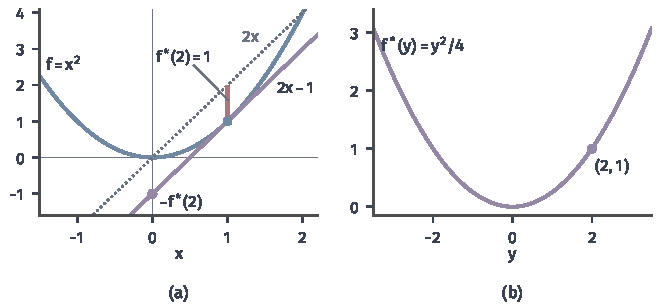
\includegraphics[width=112mm]{figures/05-optimization/06-constrained-optimization/matplotlib/dual-conj-tangent/figure.pdf}
 \caption{共轭是最高仿射下界的截距。(a)~蓝线是$f(x)=x^2$，灰色点线是$y=2$的直线$2x$，红色线段是它与$f$的最大竖直距离$f^*(2)=1$，紫线是下移后的切线，紫点是截距$-f^*(2)$。(b)~紫线是共轭函数$f^*(y)=y^2/4$，紫点对应$y=2$。}
 \label{fig:dual-conj-tangent}
\end{BookInlineFigure}

下面计算三个基本的共轭，每个都要回答一个问题：$f^*$在哪些$\bm{y}$上取有限值。

\paragraph{正定二次函数}
设$\bm{Q}\in\mathbb{R}^{n\times n}$对称正定，$f(\bm{x})=\frac12\bm{x}^\top\bm{Q}\bm{x}$。对$\bm{x}$配方，令$\bm{w}=\bm{x}-\bm{Q}^{-1}\bm{y}$，得到
\[
 \langle\bm{y},\bm{x}\rangle-\frac12\bm{x}^\top\bm{Q}\bm{x}=\frac12\bm{y}^\top\bm{Q}^{-1}\bm{y}-\frac12\bm{w}^\top\bm{Q}\bm{w}.
\]
第二项非正，在$\bm{w}=\bm{0}$时取零，于是
\begin{equation}
 f^*(\bm{y})=\frac12\bm{y}^\top\bm{Q}^{-1}\bm{y}.
 \label{eq:dual-conj-quadratic}
\end{equation}

正定性保证上确界在每个$\bm{y}$上都有限。$f(x)=x^2$相当于$Q=2$，式~\eqref{eq:dual-conj-quadratic}给出$f^*(y)=y^2/4$，$f^*(2)=1$，与图一致。

若$\bm{Q}$只是半正定，$f^*$的有限范围会缩小。例如$\mathbb{R}^2$上的$f(\bm{x})=\frac12x_1^2$，只要$y_2\neq0$，沿$x_2$方向无限走，$\langle\bm{y},\bm{x}\rangle$就趋于$+\infty$，所以$f^*(\bm{y})=+\infty$；只有$y_2=0$时，$f^*(\bm{y})=\frac12y_1^2$。

最极端的情形是线性函数$f(\bm{x})=\langle\bm{a},\bm{x}\rangle$。上确界$\sup_{\bm{x}}\langle\bm{y}-\bm{a},\bm{x}\rangle$只有$\bm{y}=\bm{a}$时有限，此时为$0$。这正是线性规划对偶中出现等式约束的原因。

\paragraph{范数}
设$\lVert\cdot\rVert$是$\mathbb{R}^n$上的一个范数。为了表述结果，先定义它的\term{对偶范数}（dual norm）：
\begin{equation}
 \lVert\bm{y}\rVert_*=\sup_{\lVert\bm{x}\rVert\leq1}\langle\bm{y},\bm{x}\rangle.
 \label{eq:dual-dual-norm}
\end{equation}
由定义，对所有$\bm{x}$，
\[
 \langle\bm{y},\bm{x}\rangle\leq\lVert\bm{y}\rVert_*\lVert\bm{x}\rVert.
\]

现在求$f(\bm{x})=\lVert\bm{x}\rVert$的共轭，分两种情形。若$\lVert\bm{y}\rVert_*\leq1$，由上式，线性项不超过范数，差值不大于零，并在$\bm{x}=\bm{0}$取到零，上确界为$0$。若$\lVert\bm{y}\rVert_*>1$，存在$\lVert\bm{x}_0\rVert\leq1$使$\langle\bm{y},\bm{x}_0\rangle>1$，于是线性项超过范数；沿$s\bm{x}_0$放大，差值随$s$线性增长，趋于$+\infty$。

合起来，范数的共轭是对偶范数单位球的约束指标函数：
\begin{equation}
 f^*(\bm{y})=\iota_{\{\lVert\bm{y}\rVert_*\leq1\}}(\bm{y}).
 \label{eq:dual-conj-norm}
\end{equation}

图~\ref{fig:dual-conj-norm}(a)和(b)是一元情形$f(x)=\lvert x\rvert$。斜率的绝对值不超过$1$的直线都能放在折线下方，斜率$1.5$的直线在$x>0$一侧无论怎样下移，最终都会越过$\lvert x\rvert$。

\paragraph{集合的约束指标函数}
设$\bm{C}$非空。由定义，
\begin{equation}
 \iota_{\bm{C}}^*(\bm{y})=\sup_{\bm{x}\in\bm{C}}\langle\bm{y},\bm{x}\rangle=:\sigma_{\bm{C}}(\bm{y}),
 \label{eq:dual-support}
\end{equation}
$\sigma_{\bm{C}}$称为$\bm{C}$的\term{支撑函数}（support function）。它回答：沿方向$\bm{y}$看，集合最远伸到哪里。集合有界时它处处有限，无界时在某些方向上可能为$+\infty$。

一元的例子是$\bm{C}=[-1,2]$。$y\geq0$时最远点是$2$，$y<0$时最远点是$-1$，所以
\[
 \sigma_{\bm{C}}(y)=\max\{2y,-y\},
\]
这是图~\ref{fig:dual-conj-norm}(c)的折线。

\begin{BookInlineFigure}
 \centering
 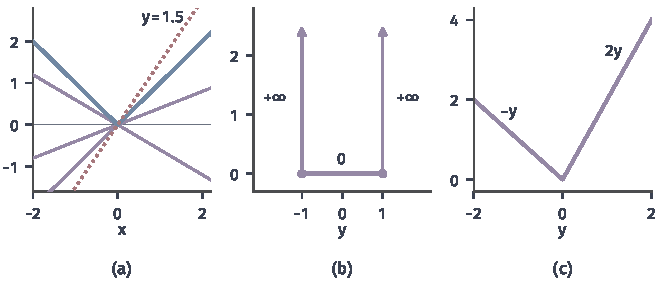
\includegraphics[width=112mm]{figures/05-optimization/06-constrained-optimization/matplotlib/dual-conj-norm/figure.pdf}
 \caption{范数与集合的共轭。(a)~蓝线是$\lvert x\rvert$，紫线是斜率$-0.6,0.4,1$的直线，都在折线下方；红色点线斜率$1.5$，不能下移成下界。(b)~$\lvert x\rvert$的共轭：在$[-1,1]$上为$0$，其余为$+\infty$。(c)~集合$[-1,2]$的支撑函数$\max\{2y,-y\}$。}
 \label{fig:dual-conj-norm}
\end{BookInlineFigure}

二维的例子能同时看到范数和支撑函数的关系。取$\bm{C}$为$\ell_1$单位球，$\bm{y}=(2,1)$。线性函数在多面体上的最大值在顶点取得，比较四个顶点$(\pm1,0),(0,\pm1)$，得到
\[
 \sigma_{\bm{C}}(\bm{y})=\max\{2,-2,1,-1\}=2=\lVert\bm{y}\rVert_\infty.
\]
一般地，$\ell_1$单位球的支撑函数就是$\ell_\infty$范数，也就是说$\ell_1$与$\ell_\infty$互为对偶范数。

图~\ref{fig:dual-support-geometry}(a)中，法向量为$\bm{y}$的直线沿$\bm{y}$方向平移，在$(1,0)$处最后一次碰到菱形。图~\ref{fig:dual-support-geometry}(b)画出了对偶范数的单位球：紫点$(0.6,0.4)$在方块内，线性项处处不超过$\ell_1$范数；红点$(1.4,0.8)$在方块外，取$\bm{x}=(1,0)$，线性项等于$1.4$，超过$\lVert\bm{x}\rVert_1=1$。

\begin{BookInlineFigure}
 \centering
 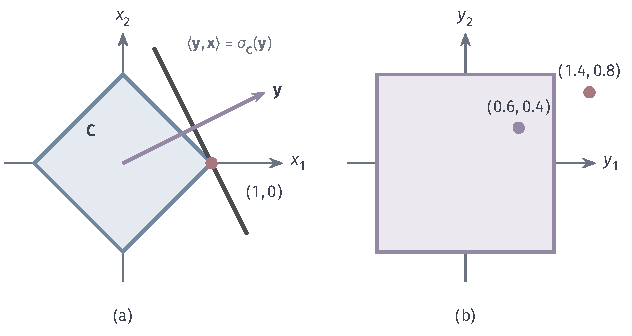
\includegraphics[width=107mm]{figures/05-optimization/06-constrained-optimization/tikz/dual-support-geometry/figure.pdf}
 \caption{支撑函数与对偶范数。(a)~浅蓝菱形是$\ell_1$单位球$\bm{C}$，紫色箭头是方向$\bm{y}=(2,1)$，深灰粗线是在红点$(1,0)$处碰到$\bm{C}$的直线$\langle\bm{y},\bm{x}\rangle=\sigma_{\bm{C}}(\bm{y})=2$。(b)~浅紫方块是$\lVert\bm{y}\rVert_\infty\leq1$，方块内的紫点使共轭为$0$，方块外的红点使共轭为$+\infty$。}
 \label{fig:dual-support-geometry}
\end{BookInlineFigure}

表~\ref{tab:dual-conjugates}汇总了这些结果，并把标量放缩算进去。这些函数常作为作用在辅助变量$\bm{z}$上的惩罚项，所以表中用$\bm{z}$和$\bm{\nu}$作变量。它显示出硬约束与软惩罚在对偶一侧的关系：硬约束$\bm{z}=\bm{0}$的乘子完全自由，二次惩罚让乘子带一个二次代价，范数惩罚让乘子落在一个球内。

\begin{BookInlineTable}
 \centering
 \begin{tabular}{@{}lll@{}}
  \toprule
  原函数$g(\bm{z})$ & 共轭$g^*(\bm{\nu})$ & 有限范围\\
  \midrule
  $\frac{\rho}{2}\lVert\bm{z}\rVert_2^2$（$\rho>0$） & $\frac{1}{2\rho}\lVert\bm{\nu}\rVert_2^2$ & 全空间\\
  $\gamma\lVert\bm{z}\rVert$（$\gamma>0$） & $\iota_{\{\lVert\bm{\nu}\rVert_*\leq\gamma\}}(\bm{\nu})$ & 对偶范数球\\
  $\iota_{\{\bm{0}\}}(\bm{z})$ & $0$ & 全空间\\
  $\iota_{\bm{C}}(\bm{z})$ & $\sigma_{\bm{C}}(\bm{\nu})$ & 由$\bm{C}$决定\\
  $\langle\bm{a},\bm{z}\rangle$ & $\iota_{\{\bm{a}\}}(\bm{\nu})$ & 单点$\bm{a}$\\
  \bottomrule
 \end{tabular}
 \caption{常用函数的共轭。第一行由式~\eqref{eq:dual-conj-quadratic}取$\bm{Q}=\rho\bm{I}$得到，第二行由式~\eqref{eq:dual-conj-norm}放缩得到。}
 \label{tab:dual-conjugates}
\end{BookInlineTable}

\subsection{共轭与最优性}
\label{sec:dual-conjugate-optimality}

共轭除了用来计算，还能描述一个点上的最优性。上确界不小于其中任何一项，由此直接得到一个不等式，它在共轭对偶中的作用，相当于弱对偶在Lagrange对偶中的作用。对任意$\bm{x}\in\operatorname{dom}f$和任意$\bm{y}$，
\begin{equation}
 f(\bm{x})+f^*(\bm{y})\geq\langle\bm{x},\bm{y}\rangle.
 \label{eq:dual-fenchel-young}
\end{equation}
这称为\term{Fenchel--Young不等式}（Fenchel--Young inequality）。

它的几何含义是：直线$\langle\bm{y},\cdot\rangle-f^*(\bm{y})$是$f$的下界，式~\eqref{eq:dual-fenchel-young}是它在$\bm{x}$处的值不超过$f(\bm{x})$。两端的差就是$\bm{x}$处$f$与这条直线之间的竖直距离。图~\ref{fig:dual-fenchel-young}(a)中$f(x)=x^2$，$x=0.5$，$y=2$，差为
\[
 0.25+1-1=0.25.
\]

什么时候取等？第~\ref{chap:nonsmooth-composite-optimization}章定义过次梯度：$\bm{y}\in\partial f(\bm{x})$是指对所有$\bm{x}'$，
\[
 f(\bm{x}')\geq f(\bm{x})+\langle\bm{y},\bm{x}'-\bm{x}\rangle.
\]
这正是说直线在$\bm{x}$处贴着$f$。

\begin{theorem}[Fenchel--Young取等条件]
 \label{thm:dual-fy-equality}
 设$f$是适当的凸函数，$\bm{x}\in\operatorname{dom}f$。则
 \begin{equation}
  \begin{aligned}
   & f(\bm{x})+f^*(\bm{y})=\langle\bm{x},\bm{y}\rangle\\
   \Longleftrightarrow\quad & \bm{y}\in\partial f(\bm{x}).
  \end{aligned}
  \label{eq:dual-fy-equality}
 \end{equation}
\end{theorem}

\begin{proof}
 由定义，左边的等式等价于$\bm{x}$达到式~\eqref{eq:dual-conjugate}中的上确界，也就是对所有$\bm{x}'\in\operatorname{dom}f$，
 \[
  \langle\bm{y},\bm{x}'\rangle-f(\bm{x}')\leq\langle\bm{y},\bm{x}\rangle-f(\bm{x}).
 \]
 移项得到
 \[
  f(\bm{x}')\geq f(\bm{x})+\langle\bm{y},\bm{x}'-\bm{x}\rangle.
 \]
 $\bm{x}'\notin\operatorname{dom}f$时这个不等式自动成立，所以它正是次梯度的定义。
\end{proof}

光滑点上次梯度只有一个，取等的$y$也只有一个，图~\ref{fig:dual-fenchel-young}(a)中$x=1$的切线斜率$2$就是这样。尖点上次梯度有多个，图~\ref{fig:dual-fenchel-young}(b)中$\lvert x\rvert$在$x=0$处，所有$y\in[-1,1]$都取等：
\[
 \lvert0\rvert+f^*(y)=0+0=0\cdot y.
\]

\begin{BookInlineFigure}
 \centering
 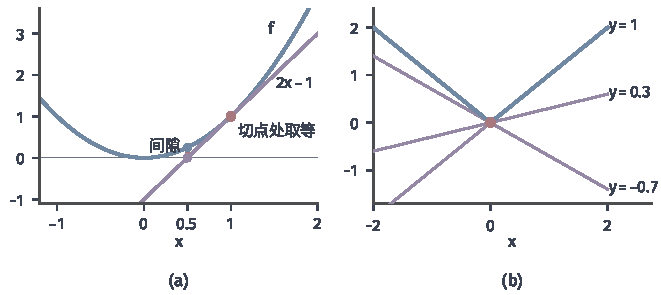
\includegraphics[width=112mm]{figures/05-optimization/06-constrained-optimization/matplotlib/dual-fenchel-young/figure.pdf}
 \caption{Fenchel--Young不等式的几何。(a)~蓝线是$f(x)=x^2$，紫线是$y=2$的最高下界$2x-1$，红色短线是$x=0.5$处的间隙$0.25$，红点$x=1$处间隙为零。(b)~蓝线是$\lvert x\rvert$，紫线是$y=-0.7,0.3,1$的下界，它们都在红点$x=0$处贴着折线，所以这些$y$都是$0$处的次梯度。}
 \label{fig:dual-fenchel-young}
\end{BookInlineFigure}

共轭把$f$变成了一族下方的直线。这些直线够不够重建$f$？把共轭再做一次，得到\term{双共轭}（biconjugate）
\begin{equation}
 f^{**}(\bm{x})=\sup_{\bm{y}}\bigl\{\langle\bm{y},\bm{x}\rangle-f^*(\bm{y})\bigr\},
 \label{eq:dual-biconjugate}
\end{equation}
它是$f$全部仿射下界的上确界。由式~\eqref{eq:dual-fenchel-young}，总有$f^{**}\leq f$。反过来的不等式需要在$f$上方的每个缺口处放进一条直线，工具是分离定理。

\begin{theorem}[点与闭凸集的严格分离]
 \label{thm:dual-separation}
 设$\bm{S}\subseteq\mathbb{R}^N$非空、闭、凸，$\bm{z}\notin\bm{S}$。则存在$\bm{a}\neq\bm{0}$和$\beta\in\mathbb{R}$，使得对所有$\bm{w}\in\bm{S}$，
 \begin{equation}
  \langle\bm{a},\bm{w}\rangle\leq\beta<\langle\bm{a},\bm{z}\rangle.
  \label{eq:dual-separation}
 \end{equation}
\end{theorem}

\begin{proof}
 第~\ref{chap:nonsmooth-composite-optimization}章已得到投影$\bm{p}=\Pi_{\bm{S}}(\bm{z})$的存在性及其刻画：
 \[
  \langle\bm{z}-\bm{p},\bm{w}-\bm{p}\rangle\leq0\qquad\text{对所有}\ \bm{w}\in\bm{S}.
 \]
 令$\bm{a}=\bm{z}-\bm{p}$，$\beta=\langle\bm{a},\bm{p}\rangle$。$\bm{z}\notin\bm{S}$而$\bm{p}\in\bm{S}$，所以$\bm{a}\neq\bm{0}$。上式就是$\langle\bm{a},\bm{w}\rangle\leq\beta$。又因为
 \[
  \langle\bm{a},\bm{z}\rangle=\beta+\lVert\bm{a}\rVert_2^2>\beta,
 \]
 式~\eqref{eq:dual-separation}成立。
\end{proof}

超平面$\{\bm{w}:\langle\bm{a},\bm{w}\rangle=\beta\}$称为\term{分离超平面}（separating hyperplane）。把分离定理用到函数上，要把函数变成集合。函数$f$的\term{上图}（epigraph）是
\[
 \operatorname{epi}f=\{(\bm{x},r):\bm{x}\in\operatorname{dom}f,\ r\geq f(\bm{x})\}.
\]
$f$凸时上图凸。$f$下半连续时上图闭：若$(\bm{x}^{(k)},r^{(k)})\to(\bm{x},r)$且$r^{(k)}\geq f(\bm{x}^{(k)})$，则$r\geq\liminf_kf(\bm{x}^{(k)})\geq f(\bm{x})$。

\begin{theorem}[Fenchel--Moreau]
 \label{thm:dual-fenchel-moreau}
 设$f:\mathbb{R}^n\to\mathbb{R}\cup\{+\infty\}$是适当、下半连续的凸函数，则$f^{**}=f$。
\end{theorem}

\begin{proof}
 已知$f^{**}\leq f$，只需证明：对任意$\bm{x}$和任意实数$r<f(\bm{x})$，存在仿射下界$\ell\leq f$使$\ell(\bm{x})>r$。因为若$\ell(\cdot)=\langle\bm{y},\cdot\rangle-\beta'$是这样的下界，由$\ell\leq f$得$f^*(\bm{y})\leq\beta'$，于是$f^{**}(\bm{x})\geq\ell(\bm{x})>r$。

 点$(\bm{x},r)$不在闭凸集$\operatorname{epi}f$中。对它应用定理~\ref{thm:dual-separation}，并把分离向量取相反数，得到$(\bm{a},b)\neq\bm{0}$和$\beta$，使对所有$(\bm{x}',r')\in\operatorname{epi}f$，
 \[
  \langle\bm{a},\bm{x}'\rangle+br'\geq\beta>\langle\bm{a},\bm{x}\rangle+br.
 \]
 上图沿$r'$向上无界，所以$b\geq0$。

 情形一：$b>0$。取$r'=f(\bm{x}')$并除以$b$，得到仿射下界
 \[
  \ell(\bm{x}')=\frac{\beta-\langle\bm{a},\bm{x}'\rangle}{b}\leq f(\bm{x}'),
 \]
 而分离的严格不等式正是$\ell(\bm{x})>r$。若$\bm{x}\in\operatorname{dom}f$，一定属于这一情形，否则$b=0$时取$\bm{x}'=\bm{x}$，$r'=f(\bm{x})$，得到矛盾：
 \[
  \langle\bm{a},\bm{x}\rangle\geq\beta>\langle\bm{a},\bm{x}\rangle.
 \]

 情形二：$b=0$，此时$\bm{x}\notin\operatorname{dom}f$，并且对所有$\bm{x}'\in\operatorname{dom}f$有$\beta-\langle\bm{a},\bm{x}'\rangle\leq0$。在$\operatorname{dom}f$中任取一点用情形一，得到某个仿射下界$\ell_0\leq f$。对$\varepsilon>0$令
 \[
  \ell_\varepsilon(\bm{x}')=\ell_0(\bm{x}')+\frac{\beta-\langle\bm{a},\bm{x}'\rangle}{\varepsilon}.
 \]
 在$\operatorname{dom}f$上第二项非正，所以$\ell_\varepsilon\leq f$。在点$\bm{x}$处$\beta-\langle\bm{a},\bm{x}\rangle>0$，$\varepsilon$足够小时$\ell_\varepsilon(\bm{x})>r$。
\end{proof}

定理的三个条件各有作用。图~\ref{fig:dual-biconjugate}(a)和(b)说明闭性的作用。$f=\iota_{(0,1)}$是凸函数，但不是下半连续的，因为端点处函数值跳到$+\infty$。它的共轭和双共轭分别是
\[
 f^*(y)=\sup_{0<x<1}xy=\max\{y,0\},\qquad f^{**}=\iota_{[0,1]}.
\]
双共轭补上了两个端点，因为仿射下界分辨不出开区间和它的闭包。

凸性的作用见图~\ref{fig:dual-biconjugate}(c)。双井函数$(x^2-1)^2$的双共轭在$[-1,1]$上是$0$，中间的鼓包被抹平了。一般地，只要$f$有仿射下界，$f^{**}$就是$f$的最大的下半连续凸下界，仿射下界只能看到函数的凸的部分。

\begin{BookInlineFigure}
 \centering
 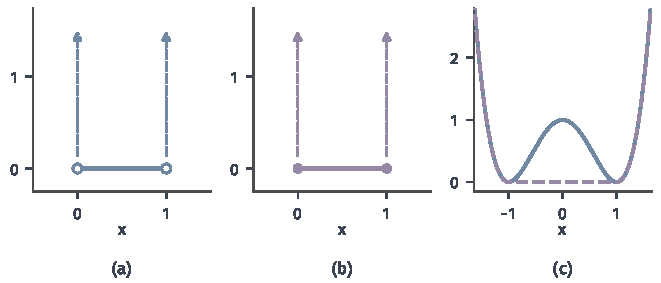
\includegraphics[width=112mm]{figures/05-optimization/06-constrained-optimization/matplotlib/dual-biconjugate/figure.pdf}
 \caption{双共轭恢复什么。(a)~$\iota_{(0,1)}$，两端的空心点表示不属于有效定义域，虚线箭头表示区间外为$+\infty$。(b)~它的双共轭$\iota_{[0,1]}$，端点变为实心。(c)~蓝线是双井函数$(x^2-1)^2$，紫色虚线是数值计算的双共轭，在$[-1,1]$上为零，在外侧与原函数重合。}
 \label{fig:dual-biconjugate}
\end{BookInlineFigure}

定理~\ref{thm:dual-fenchel-moreau}说的是一个函数可以由它的仿射下界重建，并没有说某个约束问题的对偶间隙为零。后者涉及目标和约束的联合结构，要到下一节才能回答，两件事不能混淆。

\subsection{对偶形式的推导}
\label{sec:dual-forms}

有了共轭，对偶函数可以按公式写出，不必每次重新配方。先看线性等式约束$\bm{A}\bm{x}=\bm{b}$，其中$\bm{A}\in\mathbb{R}^{p\times n}$。把内层的线性项按定义~\eqref{eq:dual-conjugate}改写：
\[
 \inf_{\bm{x}}\bigl\{f(\bm{x})+\langle\bm{A}^\top\bm{\nu},\bm{x}\rangle\bigr\}=-\sup_{\bm{x}}\bigl\{\langle-\bm{A}^\top\bm{\nu},\bm{x}\rangle-f(\bm{x})\bigr\}.
\]
右端的上确界是$f^*(-\bm{A}^\top\bm{\nu})$，于是
\begin{equation}
 q(\bm{\nu})=-f^*(-\bm{A}^\top\bm{\nu})-\bm{b}^\top\bm{\nu}.
 \label{eq:dual-q-conj}
\end{equation}

符号要逐项记住：共轭的自变量带负号，因为$\inf$变$\sup$时线性项反号。式~\eqref{eq:dual-q-conj}有限的条件是$-\bm{A}^\top\bm{\nu}\in\operatorname{dom}f^*$，也就是说，共轭的有限范围就是对偶问题的隐含约束。

用二次例核对。$\bm{Q}=\operatorname{diag}(1,4)$，$\bm{A}=(1,1)$，$b=1$。由式~\eqref{eq:dual-conj-quadratic}，
\[
 f^*(-\nu,-\nu)=\frac12\Bigl(\nu^2+\frac{\nu^2}{4}\Bigr)=\frac58\nu^2.
\]
代入式~\eqref{eq:dual-q-conj}得到$q(\nu)=-\frac58\nu^2-\nu$，与式~\eqref{eq:dual-quad-q}相同。

\paragraph{复合形式}
第~\ref{chap:nonsmooth-composite-optimization}章常见的目标是两部分之和，一部分作用在$\bm{x}$上，另一部分作用在$\bm{A}\bm{x}$上：
\begin{equation}
 \min_{\bm{x}}\ F(\bm{x})=f(\bm{x})+g(\bm{A}\bm{x}),
 \label{eq:dual-composite}
\end{equation}
其中$g:\mathbb{R}^p\to\mathbb{R}\cup\{+\infty\}$是一个函数，不是约束函数$g_i$，$\bm{A}\in\mathbb{R}^{p\times n}$。这个问题没有显式的约束，直接写Lagrange函数得不到任何东西。

办法是人为造出一条约束：引入辅助变量$\bm{z}=\bm{A}\bm{x}$，把问题改写成
\[
 \min_{\bm{x},\bm{z}}\ f(\bm{x})+g(\bm{z})\quad\text{s.t.}\quad\bm{A}\bm{x}-\bm{z}=\bm{0}.
\]
这是等价改写，最优值不变。给等式配乘子$\bm{\nu}\in\mathbb{R}^p$，Lagrange函数按$\bm{x}$和$\bm{z}$分成两部分：
\[
 \mathcal{L}=\bigl[f(\bm{x})+\langle\bm{A}^\top\bm{\nu},\bm{x}\rangle\bigr]+\bigl[g(\bm{z})-\langle\bm{\nu},\bm{z}\rangle\bigr].
\]

两部分的下确界可以分别取。第一部分和前面相同，第二部分由共轭的定义得到：
\[
 \inf_{\bm{x}}\bigl[f(\bm{x})+\langle\bm{A}^\top\bm{\nu},\bm{x}\rangle\bigr]=-f^*(-\bm{A}^\top\bm{\nu}),\qquad
 \inf_{\bm{z}}\bigl[g(\bm{z})-\langle\bm{\nu},\bm{z}\rangle\bigr]=-g^*(\bm{\nu}).
\]
于是得到\term{Fenchel对偶}（Fenchel duality）：
\begin{equation}
 \max_{\bm{\nu}}\ q(\bm{\nu})=-f^*(-\bm{A}^\top\bm{\nu})-g^*(\bm{\nu}).
 \label{eq:dual-fenchel}
\end{equation}

图~\ref{fig:dual-composite-flow}是这个推导的结构。注意$\bm{\nu}$在两项里符号相反，这是从$\bm{A}\bm{x}-\bm{z}$的两个系数来的：换成$\bm{z}-\bm{A}\bm{x}$，等于把$\bm{\nu}$换成$-\bm{\nu}$，最优值不变。

\begin{BookInlineFigure}
 \centering
 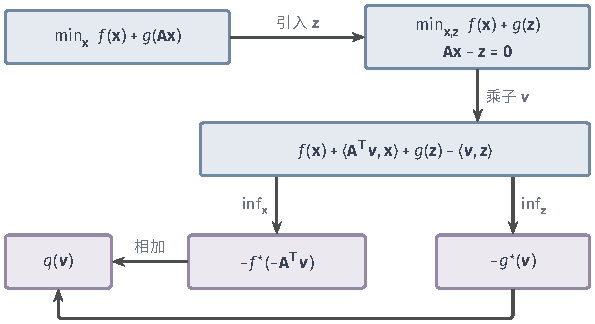
\includegraphics[width=100.8mm]{figures/05-optimization/06-constrained-optimization/tikz/dual-composite-flow/figure.pdf}
 \caption{复合问题的对偶形式怎样得到。浅蓝框是原变量一侧的表达，浅紫框是对偶一侧的量：引入$\bm{z}$，配乘子$\bm{\nu}$，再对$\bm{x}$和$\bm{z}$分别取下确界，得到两个共轭。}
 \label{fig:dual-composite-flow}
\end{BookInlineFigure}

式~\eqref{eq:dual-fenchel}的弱对偶也可以直接从Fenchel--Young不等式看出。对任意$\bm{x}$和$\bm{\nu}$，把式~\eqref{eq:dual-fenchel-young}分别用于$(f,\bm{x},-\bm{A}^\top\bm{\nu})$和$(g,\bm{A}\bm{x},\bm{\nu})$，得到
\[
 f(\bm{x})+f^*(-\bm{A}^\top\bm{\nu})\geq-\langle\bm{A}\bm{x},\bm{\nu}\rangle,\qquad
 g(\bm{A}\bm{x})+g^*(\bm{\nu})\geq\langle\bm{A}\bm{x},\bm{\nu}\rangle.
\]
两式相加，右端抵消，即得$F(\bm{x})\geq q(\bm{\nu})$。

下面算一个例子，目标沿用预算例的二次项，第二项换成绝对值惩罚：
\[
 \min_{\bm{x}\in\mathbb{R}^2}\ \frac12\bigl[(x_1-2)^2+(x_2-1)^2\bigr]+\lvert x_1+x_2\rvert.
\]
这里$\bm{A}=(1,1)$，$g=\lvert\cdot\rvert$，$\bm{a}=(2,1)$，$f(\bm{x})=\frac12\lVert\bm{x}-\bm{a}\rVert_2^2$。

先求$f^*$。上确界的驻点是$\bm{x}=\bm{a}+\bm{y}$，代入得到
\[
 f^*(\bm{y})=\langle\bm{y},\bm{a}\rangle+\frac12\lVert\bm{y}\rVert_2^2.
\]
取$\bm{y}=-\bm{A}^\top\nu=(-\nu,-\nu)$，有
\[
 f^*(-\bm{A}^\top\nu)=-3\nu+\nu^2.
\]

由表~\ref{tab:dual-conjugates}，$g^*=\iota_{[-1,1]}$，它的作用是把$\nu$限制在$[-1,1]$内。于是对偶问题是
\[
 \max_{-1\leq\nu\leq1}\ 3\nu-\nu^2.
\]
无约束最大点$\nu=3/2$在区间外，所以$\nu^\star=1$，对偶值是$3-1=2$。

回到原变量。由$\bm{x}$的驻定条件$\bm{x}-\bm{a}+\bm{A}^\top\nu=\bm{0}$，得到
\[
 \bm{x}=\bm{a}-\bm{A}^\top\nu^\star=(1,0).
\]
核对目标值：$F(1,0)=\frac12(1+1)+1=2$，等于对偶值。根据弱对偶，$(1,0)$是最优解。这里零间隙是算出来的；一般情况下式~\eqref{eq:dual-fenchel}只建立了对偶的表达，零间隙能否成立，要看下一节的条件。

\section{强对偶}
\label{sec:dual-strong}

前面的二次例、预算例和绝对值例中，最好的下界都恰好等于最优值。于是要问：这在什么时候成立？当$d^\star=f^\star$时，称\term{强对偶}成立，也说零间隙。这里有三件容易混淆的事要分开：两个最优值相等，原始最优点存在，最优乘子存在。

\paragraph{联合集合与分离}
为了看清楚乘子从哪里来，把目标和约束放到同一个空间里。定义联合集合
\begin{equation}
 \bm{A}=\bigl\{(\bm{u},\bm{w},t):\text{存在}\ \bm{x}\in\bm{D}\ \text{使}\ g_i(\bm{x})\leq u_i,\ h_j(\bm{x})=w_j,\ f(\bm{x})\leq t\bigr\}.
 \label{eq:dual-joint-set}
\end{equation}
$(\bm{u},\bm{w})$是约束右端允许的松动量，$t$是能够达到的目标值。原问题的最优值是集合$\bm{A}$在$(\bm{u},\bm{w})=\bm{0}$这条竖线上的最低高度。

$\bm{\lambda}\geq\bm{0}$时，对偶函数可以用这个集合重写：
\[
 q(\bm{\lambda},\bm{\nu})=\inf_{(\bm{u},\bm{w},t)\in\bm{A}}\bigl\{t+\langle\bm{\lambda},\bm{u}\rangle+\langle\bm{\nu},\bm{w}\rangle\bigr\}.
\]
所以$q$是用法向量$(\bm{\lambda},\bm{\nu},1)$的超平面从下方托住$\bm{A}$时，在竖轴上的高度。$f,g_i$凸且$h_j$仿射时$\bm{A}$是凸集，分离定理就有了用武之地。

设想把一张纸从下方贴到$\bm{A}$上，碰在点$(\bm{0},f^\star)$处。如果纸不是竖直的，就可以把法向量的$t$分量归一成$1$，其余分量就是乘子，竖轴上的高度就是$f^\star$，强对偶成立。所以问题的关键是这张纸是否竖直。

图~\ref{fig:dual-joint-set}对比两种情形，只有一条不等式，$\bm{A}$位于平面上。(a)是一元例，$\bm{A}$的下边界是最优值函数$v(u)=\frac12\max\{1-u,0\}^2$。它在$u=0$的两侧都有定义，切线$t=\frac12-u$的斜率给出$\lambda^\star=1$。

(b)是问题$\min x$，约束$x^2\leq u$。$u<0$时不可行，$v(u)=-\sqrt{u}$在$u=0$处切线竖直。能托住$\bm{A}$并经过原点的只有竖直线，它不对应任何有限的乘子。

\begin{BookInlineFigure}
 \centering
 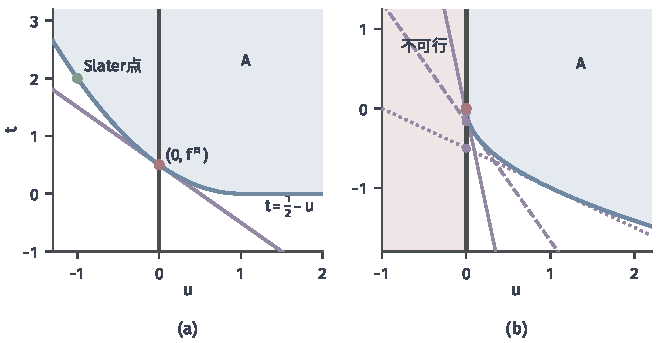
\includegraphics[width=112mm]{figures/05-optimization/06-constrained-optimization/matplotlib/dual-joint-set/figure.pdf}
 \caption{联合集合$\bm{A}$（浅蓝）与托住它的直线。(a)~一元例：紫线$t=\frac12-u$在红点$(0,f^\star)$处托住$\bm{A}$，斜率对应$\lambda^\star=1$；绿点是Slater点$x=0$对应的$(g,f)=(-1,2)$，它在竖线$u=0$的左侧。(b)~$\min x$，约束$x^2\leq u$：浅红区域$u<0$不可行，$\bm{A}$的边界在红点处切线竖直，紫线是$\lambda=0.5,1.5,5$（点线、虚线、实线）的托线，交点高度$-1/(4\lambda)$随$\lambda$增大升向$0$，但能经过红点的只有深灰色竖线。}
 \label{fig:dual-joint-set}
\end{BookInlineFigure}

要排除竖直的纸，只需要$\bm{A}$在竖线左侧确实有点，这正是图~\ref{fig:dual-joint-set}(a)中绿点起的作用。

\subsection{Slater条件}
\label{sec:dual-slater}

把上面的想法写成条件。设$f,g_i:\mathbb{R}^n\to\mathbb{R}\cup\{+\infty\}$是凸函数，等式约束仿射，写成$\bm{A}\bm{x}=\bm{b}$，其中$\bm{A}\in\mathbb{R}^{p\times n}$。共同有效定义域是
\[
 \bm{D}=\operatorname{dom}f\cap\bigcap_i\operatorname{dom}g_i.
\]
第~\ref{chap:nonsmooth-composite-optimization}章用$\operatorname{ri}$表示相对内部，即在集合自身的仿射包内的内点。

\begin{definition}[Slater条件]
 \label{def:dual-slater}
 若存在$\bar{\bm{x}}\in\operatorname{ri}\bm{D}$，使
 \begin{equation}
  g_i(\bar{\bm{x}})<0,\quad i=1,\ldots,m,\qquad\bm{A}\bar{\bm{x}}=\bm{b},
  \label{eq:dual-slater}
 \end{equation}
 就称问题满足\term{Slater条件}（Slater's condition），$\bar{\bm{x}}$称为Slater点。
\end{definition}

条件的每一部分都有用处。严格不等式让点落在竖线左侧；等式约束无法严格，只要求满足；取在相对内部，是为了让定义域在$\bar{\bm{x}}$周围留有余地，否则余量可能恰好被定义域的边缘吃掉。

三个例子都容易找到Slater点。一元例取$\bar{x}=0$，$g(\bar{x})=-1<0$。预算例取$\bar{\bm{x}}=(1/2,1/2)$，它在$\bm{D}=\mathbb{R}^2_{+}$的内部，且$x_1+x_2-2=-1<0$。二次例没有不等式，取约束直线上的任一点。

证明要分离的不是闭集，$(\bm{0},f^\star)$可能就在$\bm{A}$的边界上。定理~\ref{thm:dual-separation}不够用，需要下面这个不要求闭性、也不要求严格的版本。

\begin{lemma}[点与凸集的分离]
 \label{lem:dual-separation-convex}
 设$\bm{S}\subseteq\mathbb{R}^N$非空、凸，$\bm{z}\notin\bm{S}$。则存在$\bm{a}\neq\bm{0}$，使得对所有$\bm{w}\in\bm{S}$，
 \begin{equation}
  \langle\bm{a},\bm{w}\rangle\geq\langle\bm{a},\bm{z}\rangle.
  \label{eq:dual-separation-convex}
 \end{equation}
\end{lemma}

\begin{proof}
 $\mathbb{R}^N$的子集有可数稠密子集，取$\bm{S}$中的这样一列点$\bm{w}_1,\bm{w}_2,\ldots$。对每个$k$，令$\bm{S}_k$是$\bm{w}_1,\ldots,\bm{w}_k$的凸组合全体。

 $\bm{S}_k$是单纯形在连续映射下的像，所以是紧的，从而是闭集；它包含于凸集$\bm{S}$，所以不含$\bm{z}$。对$\bm{S}_k$用定理~\ref{thm:dual-separation}，取相反数并归一化，得到单位向量$\bm{a}_k$，使
 \[
  \langle\bm{a}_k,\bm{w}_j\rangle>\langle\bm{a}_k,\bm{z}\rangle,\qquad j=1,\ldots,k.
 \]

 单位球面是紧集，$\bm{a}_k$有收敛子列，极限$\bm{a}$仍是单位向量。固定$j$，让$k$沿子列趋于无穷，得到
 \[
  \langle\bm{a},\bm{w}_j\rangle\geq\langle\bm{a},\bm{z}\rangle.
 \]
 $\{\bm{w}_j\}$在$\bm{S}$中稠密，内积连续，所以式~\eqref{eq:dual-separation-convex}对全部$\bm{w}\in\bm{S}$成立。
\end{proof}

\begin{theorem}[Slater条件下的强对偶]
 \label{thm:dual-slater}
 设问题的$f,g_i$凸、等式约束仿射，满足Slater条件，且$f^\star$有限。则
 \begin{equation}
  d^\star=f^\star,
  \label{eq:dual-strong}
 \end{equation}
 并且对偶最优值被某组$(\bm{\lambda}^\star,\bm{\nu}^\star)$达到，其中$\bm{\lambda}^\star\geq\bm{0}$。
\end{theorem}

\begin{proof}
 第一步，选取工作空间。令$\bm{V}$是$\bm{D}$的仿射包的方向子空间，$\bm{W}=\{\bm{A}\bm{v}:\bm{v}\in\bm{V}\}$。对$\bm{x}\in\bm{D}$，由$\bm{A}\bar{\bm{x}}=\bm{b}$，有
 \[
  \bm{A}\bm{x}-\bm{b}=\bm{A}(\bm{x}-\bar{\bm{x}})\in\bm{W}.
 \]
 所以等式残差不会离开$\bm{W}$，只需要在$\mathbb{R}^m\times\bm{W}\times\mathbb{R}$中讨论。

 第二步，构造被分离的集合。令$\bm{S}$是满足下面条件的$(\bm{u},\bm{w},t)$的全体：存在$\bm{x}\in\bm{D}$，使$g_i(\bm{x})\leq u_i$，$\bm{A}\bm{x}-\bm{b}=\bm{w}$，$f(\bm{x})<t$。由$f,g_i$的凸性和等式的仿射性，$\bm{S}$是凸集，并且它是非空的，因为$\bar{\bm{x}}\in\bm{D}$。点$(\bm{0},\bm{0},f^\star)$不在$\bm{S}$中，否则存在可行点使$f(\bm{x})<f^\star$。

 第三步，应用分离。由引理~\ref{lem:dual-separation-convex}，存在不全为零的$\bm{\lambda}\in\mathbb{R}^m$、$\bm{\nu}\in\bm{W}$、$\lambda_0\in\mathbb{R}$，使对所有$(\bm{u},\bm{w},t)\in\bm{S}$，
 \[
  \langle\bm{\lambda},\bm{u}\rangle+\langle\bm{\nu},\bm{w}\rangle+\lambda_0t\geq\lambda_0f^\star.
 \]
 $\bm{S}$中的点可以把$u_i$或$t$任意增大，若$\lambda_i<0$或$\lambda_0<0$，左端会趋于$-\infty$，所以$\bm{\lambda}\geq\bm{0}$，$\lambda_0\geq0$。

 任取$\bm{x}\in\bm{D}$，取$\bm{u}=(g_i(\bm{x}))_i$，$\bm{w}=\bm{A}\bm{x}-\bm{b}$，$t=f(\bm{x})+\varepsilon$，令$\varepsilon\downarrow0$，得到
 \[
  \sum_i\lambda_ig_i(\bm{x})+\langle\bm{\nu},\bm{A}\bm{x}-\bm{b}\rangle+\lambda_0f(\bm{x})\geq\lambda_0f^\star,\qquad\bm{x}\in\bm{D}.
 \]

 第四步，证明$\lambda_0>0$，也就是这张纸不竖直。设$\lambda_0=0$。把$\bm{x}=\bar{\bm{x}}$代入上式，等式项为零，得到
 \[
  \sum_i\lambda_ig_i(\bar{\bm{x}})\geq0.
 \]
 由$g_i(\bar{\bm{x}})<0$和$\bm{\lambda}\geq\bm{0}$，只能$\bm{\lambda}=\bm{0}$。于是$\bm{\nu}\neq\bm{0}$，并且上式变成对所有$\bm{x}\in\bm{D}$，
 \[
  \langle\bm{\nu},\bm{A}(\bm{x}-\bar{\bm{x}})\rangle\geq0.
 \]
 因为$\bar{\bm{x}}\in\operatorname{ri}\bm{D}$，存在$r>0$，使对$\bm{v}\in\bm{V}$，$\lVert\bm{v}\rVert_2\leq r$，都有$\bar{\bm{x}}+\bm{v}\in\bm{D}$。代入$\pm\bm{v}$，得到$\langle\bm{\nu},\bm{A}\bm{v}\rangle=0$，也就是$\bm{\nu}$与$\bm{W}$正交。而$\bm{\nu}\in\bm{W}$，所以$\bm{\nu}=\bm{0}$，矛盾。

 第五步，构造乘子。令$\bm{\lambda}^\star=\bm{\lambda}/\lambda_0$，$\bm{\nu}^\star=\bm{\nu}/\lambda_0$，除以$\lambda_0$，上面第三步的不等式成为对所有$\bm{x}\in\bm{D}$，
 \[
  \mathcal{L}(\bm{x},\bm{\lambda}^\star,\bm{\nu}^\star)\geq f^\star.
 \]
 对$\bm{x}$取下确界，
 \[
  q(\bm{\lambda}^\star,\bm{\nu}^\star)\geq f^\star.
 \]
 由弱对偶，
 \[
  q(\bm{\lambda}^\star,\bm{\nu}^\star)\leq d^\star\leq f^\star.
 \]
 所以三者相等，并且这组乘子达到$d^\star$。
\end{proof}

证明里Slater点只在第四步用到，这正是前面“排除竖直的纸”的严格写法。定理的结论并不包括原始最优点存在，这一点在第~\ref{sec:dual-gap-attainment}节用例子说明。Slater点本身可行，所以$f^\star<+\infty$，有限的假设只是排除$f^\star=-\infty$；这时弱对偶迫使$d^\star=-\infty$，对偶可行的乘子不存在，也就谈不上最优乘子。

如果某些$g_i$本身是仿射的，这些约束不必严格满足，只要$g_i(\bar{\bm{x}})\leq0$，其余要求不变。原因在于仿射约束的集合是多面体，分离时不会出现图~\ref{fig:dual-joint-set}(b)那样切线竖直的边缘，这与线性规划不需要严格可行点的道理相同。证明需要用到多面体凸集的分离，篇幅较长，读者可查阅\scite{rockafellar1970convex}。全部约束都仿射、目标线性时，这就是第~\ref{chap:linear-programming}章已经证明的强对偶。

\subsection{共轭对偶的正则条件}
\label{sec:dual-regularity}

复合问题~\eqref{eq:dual-composite}没有不等式，不等式上的“严格可行”没有对应物，正则条件要换一种说法。回忆它的改写形式：变量$(\bm{x},\bm{z})$，有效定义域是$\operatorname{dom}f\times\operatorname{dom}g$，约束是线性等式。Slater条件要求的是存在满足等式、位于定义域相对内部的点。乘积集的仿射包是各因子仿射包的乘积，所以乘积集的相对内部等于各因子相对内部的乘积，这就翻译成了下面的条件。

\begin{theorem}[Fenchel对偶的强对偶]
 \label{thm:dual-fenchel-strong}
 设$f:\mathbb{R}^n\to\mathbb{R}\cup\{+\infty\}$，$g:\mathbb{R}^p\to\mathbb{R}\cup\{+\infty\}$是适当、下半连续的凸函数，$\bm{A}\in\mathbb{R}^{p\times n}$。若存在$\bm{x}$使
 \begin{equation}
  \bm{x}\in\operatorname{ri}(\operatorname{dom}f),\qquad\bm{A}\bm{x}\in\operatorname{ri}(\operatorname{dom}g),
  \label{eq:dual-fenchel-regular}
 \end{equation}
 且式~\eqref{eq:dual-composite}的最优值$F^\star$有限，则$\sup_{\bm{\nu}}q(\bm{\nu})=F^\star$，其中$q$由式~\eqref{eq:dual-fenchel}给出，并且对偶最优值被达到。
\end{theorem}

\begin{proof}
 把定理~\ref{thm:dual-slater}用于改写形式，变量是$(\bm{x},\bm{z})$，目标是$f(\bm{x})+g(\bm{z})$，等式是$\bm{A}\bm{x}-\bm{z}=\bm{0}$，没有不等式。若$\bm{x}$满足式~\eqref{eq:dual-fenchel-regular}，则$(\bm{x},\bm{A}\bm{x})$在定义域的相对内部且满足等式，是Slater点。改写形式的对偶函数正是式~\eqref{eq:dual-fenchel}。
\end{proof}

证明中没有用到下半连续。这个假设保证$f^{**}=f$和$g^{**}=g$，使$q$对应的对偶问题再取一次对偶时能回到原问题，所以通常写在一起。定理保证的是两个最优值相等、对偶最优乘子存在，原始问题的最小点是否存在，要另外用强制性或紧性论证。

上一节的绝对值例中$\operatorname{dom}f=\mathbb{R}^2$，$\operatorname{dom}g=\mathbb{R}$，两个定义域都是全空间，条件自动满足，所以那里的零间隙在算出结果之前就可以预知。

条件中的相对内部不是形式要求，看一个定义域只在边界上相遇的例子。取$f(x)=-\sqrt{x}$（$x\geq0$，其余为$+\infty$），$g=\iota_{\{0\}}$，$A=1$。此时要求$x\in(0,\infty)$且$x=0$，式~\eqref{eq:dual-fenchel-regular}不成立。可行点只有$x=0$，所以$F^\star=0$。

对偶一侧，$g^*=0$。$\nu>0$时$f^*(-\nu)=\sup_{x\geq0}\{-\nu x+\sqrt{x}\}$在$\sqrt{x}=1/(2\nu)$处达到，于是
\[
 f^*(-\nu)=\frac{1}{4\nu},\qquad q(\nu)=-\frac{1}{4\nu}.
\]
$\nu\leq0$时$f^*(-\nu)=+\infty$。所以$\sup q=0=F^\star$，零间隙仍然成立，但上确界取不到，对偶最优乘子不存在。

\subsection{间隙与达到的区别}
\label{sec:dual-gap-attainment}

“强对偶成立”“原始最优点存在”“最优乘子存在”是三件不同的事。本小节用三个例子分别让其中一件出问题，表~\ref{tab:dual-gap-cases}是它们的汇总。

第一个例子最小化$e^{-x}$，约束$-x\leq0$。Slater点$x=1$存在，$f^\star=0$有限，定理~\ref{thm:dual-slater}适用。第~\ref{sec:dual-function}节已经算出$q(0)=0$，其余$q(\lambda)=-\infty$，于是
\[
 d^\star=0=f^\star,\qquad\lambda^\star=0.
\]
零间隙成立，乘子达到，但没有$x$能使$e^{-x}=0$，原始最优值不达到。图~\ref{fig:dual-three-failures}(a)是这个函数，它只在无穷远处靠近下确界。

第二个例子最小化$x$，约束$x^2\leq0$。唯一的可行点是$x=0$，所以$f^\star=0$，原始最优点存在。Slater条件不成立，因为$x^2<0$无解。

对$\lambda>0$，$x+\lambda x^2$在$x=-1/(2\lambda)$处最小，$\lambda=0$时下确界为$-\infty$。于是
\[
 q(\lambda)=-\frac{1}{4\lambda}\quad(\lambda>0).
\]
$\lambda\to+\infty$时$q\to0$，所以$d^\star=0=f^\star$，零间隙成立，但没有有限的$\lambda$能达到。如图~\ref{fig:dual-three-failures}(b)，这正是图~\ref{fig:dual-joint-set}(b)中切线竖直的代价。

这个例子还说明，第~\ref{chap:constrained-optimality}章在同一问题上看到的“最小点没有KKT乘子”，与“对偶最优值取不到”是同一件事的两面。

第三个例子的定义域是$\bm{D}=\{\bm{x}\in\mathbb{R}^2:x_2>0\}$，问题是
\[
 \min_{\bm{x}\in\bm{D}}\ e^{-x_1}\quad\text{s.t.}\quad\frac{x_1^2}{x_2}\leq0.
\]
函数$x_1^2/x_2$在$x_2>0$上是凸的，这可以由Hessian半正定验证，所以这是一个凸问题。约束迫使$x_1=0$，于是$f^\star=1$，并在$\{0\}\times(0,\infty)$上达到。

求对偶函数。对任意$\lambda\geq0$，内层函数$e^{-x_1}+\lambda x_1^2/x_2$总是正的，所以$q(\lambda)\geq0$。沿曲线$x_1=s$，$x_2=s^3$，令$s\to+\infty$，有
\[
 e^{-s}+\frac{\lambda}{s}\to0.
\]
所以$q(\lambda)=0$对所有$\lambda\geq0$成立，$d^\star=0$。

两个最优值分别是$1$和$0$，对偶间隙为$1$。这说明凸性本身不能保证零间隙。Slater条件在这里失败，因为$x_1^2/x_2<0$无解。

图~\ref{fig:dual-three-failures}(c)显示了联合集合的样子：最优值函数$v$在$u=0$处的值是$1$，而$u>0$时只要让$x_1,x_2$都增大，就有$x_1^2/x_2\leq u$，目标值可以任意接近$0$，所以$v(u)=0$。$v$在$u=0$处有一个跳跃，从下方托住$\bm{A}$的直线最高只能到$0$。

\begin{BookInlineFigure}
 \centering
 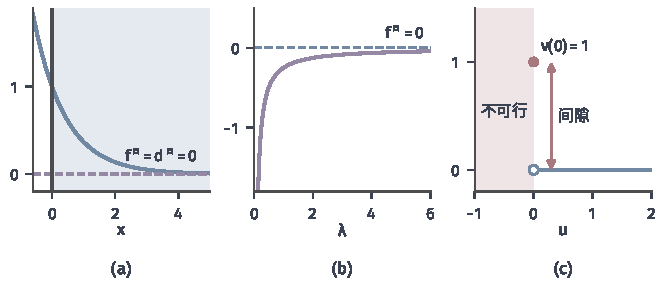
\includegraphics[width=112mm]{figures/05-optimization/06-constrained-optimization/matplotlib/dual-three-failures/figure.pdf}
 \caption{三种不同的情形。(a)~蓝线是$e^{-x}$，浅蓝区域可行，下确界$0$不被取到，紫色虚线是$d^\star$。(b)~$\min x$，约束$x^2\leq0$的对偶函数$q(\lambda)=-1/(4\lambda)$，向蓝色虚线$f^\star=0$靠近但取不到。(c)~第三个例子的最优值函数：浅红区域$u<0$不可行，红点是$v(0)=1$，$u>0$时$v(u)=0$，空心点表示$u=0$时下极限，红色箭头是对偶间隙$1$。}
 \label{fig:dual-three-failures}
\end{BookInlineFigure}

\begin{BookInlineTable}
 \centering
 \begin{tabular}{@{}llllll@{}}
  \toprule
  问题 & Slater & $f^\star$ & $d^\star$ & 原始达到 & 对偶达到\\
  \midrule
  $\min e^{-x}$，$-x\leq0$ & 成立 & $0$ & $0$ & 否 & 是\\
  $\min x$，$x^2\leq0$ & 不成立 & $0$ & $0$ & 是 & 否\\
  $\min e^{-x_1}$，$x_1^2/x_2\leq0$ & 不成立 & $1$ & $0$ & 是 & 是\\
  \bottomrule
 \end{tabular}
 \caption{间隙与达到的三个例子。第三个例子全部乘子都是对偶最优的。}
 \label{tab:dual-gap-cases}
\end{BookInlineTable}

表中第二行和第三行都不满足Slater条件，结局却不同：一个零间隙，一个正间隙。所以Slater条件只是充分条件，不成立时要具体分析。

\section{最优性证书}
\label{sec:dual-certificates}

前面分别得到了下界、KKT条件和强对偶。接下来要弄清：手上有一对原始—对偶候选，怎样判断它已经解决了原问题，这几种工具各自检验了什么？

先看一个不能只信对偶一侧的例子。设$\bm{D}=[0,1]$，
\[
 \min_{x\in[0,1]}\ -x\quad\text{s.t.}\quad x-\frac12\leq0.
\]
目标要求$x$尽量大，约束限制$x$不超过$1/2$，所以解是$x^\star=1/2$，$f^\star=-1/2$。Lagrange函数对$x$是线性的，下确界在$\bm{D}$的端点取得，比较$x=0$和$x=1$两处的值，得到
\[
 q(\lambda)=\min\Bigl\{-\frac{\lambda}{2},\ \frac{\lambda}{2}-1\Bigr\}.
\]

$\lambda^\star=1$是这条折线的最高点，$q(1)=-1/2=f^\star$，强对偶成立。一个只盯着对偶目标的算法到这里就停止了。但它手里的原变量是内层的最小点：$\lambda<1$时是$x=1$，$\lambda>1$时是$x=0$，如图~\ref{fig:dual-recover-fail}(b)所示。

$x=1$不可行，$x=0$可行但目标值是$0$，比$f^\star$差。$\lambda=1$时内层的最小点是整个$[0,1]$，$x^\star$只是其中一点，内层本身挑不出它。所以乘子停止改进不等于原问题解完了，求出的候选必须回到原问题上检验。

\begin{BookInlineFigure}
 \centering
 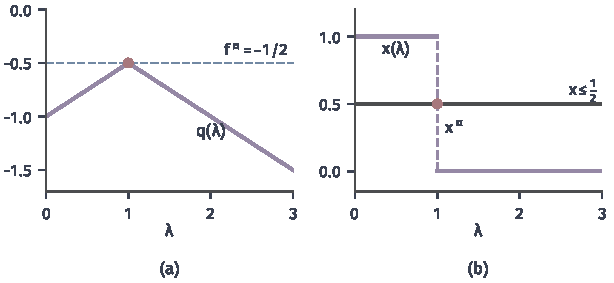
\includegraphics[width=104mm]{figures/05-optimization/06-constrained-optimization/matplotlib/dual-recover-fail/figure.pdf}
 \caption{对偶最优不等于得到了原始解。(a)~紫线是折线$q(\lambda)$，红点是对偶最优点$\lambda^\star=1$，蓝色虚线是$f^\star$。(b)~紫线是内层最小点$x(\lambda)$，它在$\lambda=1$处从$1$跳到$0$，紫色虚线表示此时最小点是整个区间；深灰粗线是约束边界，红点是$x^\star$，内层解不会自动落到它上面。}
 \label{fig:dual-recover-fail}
\end{BookInlineFigure}

\subsection{零间隙与KKT}
\label{sec:dual-zero-gap-kkt}

可以检验的证据是一对候选加上零间隙。第~\ref{chap:constrained-optimality}章的KKT条件是在候选点$\bm{x}$处的四组关系：$\bm{x}$可行；$\bm{\lambda}\geq\bm{0}$；互补松弛$\lambda_ig_i(\bm{x})=0$；以及Lagrange函数对$\bm{x}$驻定，
\[
 \nabla f(\bm{x})+\sum_i\lambda_i\nabla g_i(\bm{x})+\sum_j\nu_j\nabla h_j(\bm{x})=\bm{0}.
\]
那里证明了，凸问题的KKT点是全局最小点。下面把这个结论与零间隙联系起来。

\begin{theorem}[零间隙与KKT]
 \label{thm:dual-zero-gap-kkt}
 考虑问题~\eqref{eq:dual-primal}。

 第一，设$\bm{x}^\star$可行，$\bm{\lambda}^\star\geq\bm{0}$，且
 \begin{equation}
  f(\bm{x}^\star)=q(\bm{\lambda}^\star,\bm{\nu}^\star).
  \label{eq:dual-zero-gap}
 \end{equation}
 则$\bm{x}^\star$原始全局最优，$(\bm{\lambda}^\star,\bm{\nu}^\star)$对偶最优，互补松弛成立，并且$\bm{x}^\star$在$\bm{D}$上全局最小化$\mathcal{L}(\cdot,\bm{\lambda}^\star,\bm{\nu}^\star)$。若各函数在$\bm{x}^\star$处可微且$\bm{x}^\star\in\operatorname{int}\bm{D}$，则$(\bm{x}^\star,\bm{\lambda}^\star,\bm{\nu}^\star)$满足KKT条件。

 第二，设$\bm{D}$是开凸集，$f,g_i$在其上凸且可微，$h_j$仿射，$(\bm{x}^\star,\bm{\lambda}^\star,\bm{\nu}^\star)$满足KKT条件。则式~\eqref{eq:dual-zero-gap}成立，原始、对偶两侧都最优。
\end{theorem}

\begin{proof}
 第一部分。由弱对偶，
 \[
  f(\bm{x}^\star)=q(\bm{\lambda}^\star,\bm{\nu}^\star)\leq d^\star\leq f^\star\leq f(\bm{x}^\star),
 \]
 各处取等，所以两侧都最优。

 再写一条链，由$q$的定义和可行性，
 \[
  q(\bm{\lambda}^\star,\bm{\nu}^\star)\leq\mathcal{L}(\bm{x}^\star,\bm{\lambda}^\star,\bm{\nu}^\star)=f(\bm{x}^\star)+\sum_i\lambda_i^\star g_i(\bm{x}^\star)\leq f(\bm{x}^\star).
 \]
 两端相等，所以两个不等号都取等。第二个不等号取等给出
 \[
  \sum_i\lambda_i^\star g_i(\bm{x}^\star)=0.
 \]
 每一项非正，因此每一项都是零，这就是互补松弛。

 第一个不等号取等，说明$\mathcal{L}(\bm{x}^\star,\bm{\lambda}^\star,\bm{\nu}^\star)$等于它在$\bm{D}$上的下确界，即$\bm{x}^\star$是全局最小点。若$\bm{x}^\star$是$\bm{D}$的内点且函数可微，梯度为零就是驻定条件。

 第二部分。$\lambda_i^\star\geq0$且$h_j$仿射，所以$\mathcal{L}(\cdot,\bm{\lambda}^\star,\bm{\nu}^\star)$在$\bm{D}$上是凸函数，驻点就是全局最小点。于是由互补松弛和可行性，
 \[
  q(\bm{\lambda}^\star,\bm{\nu}^\star)=\mathcal{L}(\bm{x}^\star,\bm{\lambda}^\star,\bm{\nu}^\star)=f(\bm{x}^\star).
 \]
 再用第一部分即得结论。
\end{proof}

定理的第一部分不要求凸性，这是最通用的最优性证据，并且把KKT作为一个推论给出来。用预算例核对：$\bm{x}^\star=(3/2,1/2)$可行，$\lambda^\star=1/2$，由式~\eqref{eq:dual-budget-q}有$q(1/2)=1/4=f(\bm{x}^\star)$，所以这一对候选的最优性得到了证明，不需要知道解是怎样算出来的。

反过来就要小心了。非凸问题的Lagrange驻定不代表内层全局最小，定理第二部分的凸性假设不能省略。看$\min-x^2$，约束$x-1\leq0$和$-x-1\leq0$。图~\ref{fig:dual-nonconvex-kkt}(a)标出了三个KKT点：$x=0$（乘子全为零）和$x=\pm1$。

$x=0$的目标值是$0$，它甚至是一个局部最大点，KKT只把它列为候选。$x=1$是真正的全局最小点，由驻定条件$-2+\lambda_1=0$得$\lambda_1=2$，$\lambda_2=0$。此时
\[
 \mathcal{L}(x,2,0)=-x^2+2(x-1)=-(x-1)^2-1.
\]
这条开口向下的抛物线在$x=1$处是\emph{最大}点，如图~\ref{fig:dual-nonconvex-kkt}(b)。$q(2,0)=-\infty$，这一对KKT候选的候选间隙是$+\infty$。

所以即便$x=1$确实最优，这组乘子也给不出证书。换一种约束写法，结果又不同。把可行集写成$x^2-1\leq0$，则
\[
 \mathcal{L}(x,\lambda)=(\lambda-1)x^2-\lambda,\qquad q(\lambda)=-\lambda\quad(\lambda\geq1).
\]
$\lambda=1$时$q=-1=f^\star$，零间隙成立。可行集完全相同，对偶却依赖约束的写法，这也是非凸问题的一个特点。

\begin{BookInlineFigure}
 \centering
 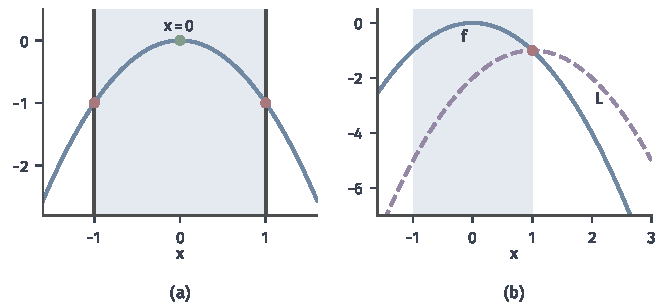
\includegraphics[width=112mm]{figures/05-optimization/06-constrained-optimization/matplotlib/dual-nonconvex-kkt/figure.pdf}
 \caption{非凸问题的KKT点不等于零间隙候选。(a)~$\min-x^2$，浅蓝区域是$[-1,1]$，红点是全局最优点$x=\pm1$，绿点是KKT点$x=0$，它是局部最大点。(b)~蓝线是$f$，紫色虚线是$\mathcal{L}(\cdot,2,0)=-(x-1)^2-1$，它在红点$x=1$处驻定，但那里是最大点，$\mathcal{L}$没有下界。}
 \label{fig:dual-nonconvex-kkt}
\end{BookInlineFigure}

\subsection{Lagrange鞍点}
\label{sec:dual-saddle}

上面的证书也可以用一个不等式组写出，它把原始和对偶两个问题放在对称的位置上。关键的一步，是发现原问题本身也能用$\mathcal{L}$写出来。固定$\bm{x}\in\bm{D}$，对乘子取上确界：
\begin{equation}
 \sup_{\bm{\lambda}\geq\bm{0},\ \bm{\nu}}\mathcal{L}(\bm{x},\bm{\lambda},\bm{\nu})=\begin{cases}f(\bm{x}), & \bm{x}\ \text{可行},\\+\infty, & \bm{x}\ \text{不可行}.\end{cases}
 \label{eq:dual-sup-recovers}
\end{equation}

理由是：若某条$g_i(\bm{x})>0$，令$\lambda_i\to+\infty$；若某条$h_j(\bm{x})\neq0$，令$\nu_j\to\pm\infty$，都趋于$+\infty$。若$\bm{x}$可行，$\lambda_ig_i\leq0$且$\nu_jh_j=0$，取$\bm{\lambda}=\bm{0}$就达到上确界$f(\bm{x})$。这就是开头说的“硬墙”：把价格抬到无穷大，就重新得到了硬约束。

所以原问题是$\inf_{\bm{x}}\sup_{\bm{\lambda},\bm{\nu}}\mathcal{L}$，对偶问题是$\sup_{\bm{\lambda},\bm{\nu}}\inf_{\bm{x}}\mathcal{L}$，两者只差取极值的次序，弱对偶正是一般的不等式$\sup\inf\leq\inf\sup$。图~\ref{fig:dual-saddle}(b)用一元例画出了式~\eqref{eq:dual-sup-recovers}：$x=0$可行，直线随$\lambda$下降，上确界在$\lambda=0$处取到$f(0)=2$；$x=1.5$不可行，直线向上趋于无穷。

\begin{definition}[Lagrange鞍点]
 \label{def:dual-saddle}
 设$\bm{x}^\star\in\bm{D}$，$\bm{\lambda}^\star\geq\bm{0}$。若对所有$\bm{x}\in\bm{D}$、$\bm{\lambda}\geq\bm{0}$、$\bm{\nu}$都有
 \begin{equation}
  \mathcal{L}(\bm{x}^\star,\bm{\lambda},\bm{\nu})\leq\mathcal{L}(\bm{x}^\star,\bm{\lambda}^\star,\bm{\nu}^\star)\leq\mathcal{L}(\bm{x},\bm{\lambda}^\star,\bm{\nu}^\star),
  \label{eq:dual-saddle}
 \end{equation}
 就称$(\bm{x}^\star,\bm{\lambda}^\star,\bm{\nu}^\star)$是\term{Lagrange鞍点}（Lagrangian saddle point）。
\end{definition}

式~\eqref{eq:dual-saddle}的右半边是全局最小，不是局部驻定，这是它与KKT的关键区别。图~\ref{fig:dual-saddle}(a)是一元例中$\mathcal{L}(x,\lambda)$的等高线，$(1,1)$是鞍点。沿绿色虚线（固定$\lambda=1$）$\mathcal{L}$在$x=1$处最小，见图~\ref{fig:dual-saddle}(c)；沿紫色虚线（固定$x=1$）$\mathcal{L}$恒为$\frac12$，这时左半边取等。

\begin{BookInlineFigure}
 \centering
 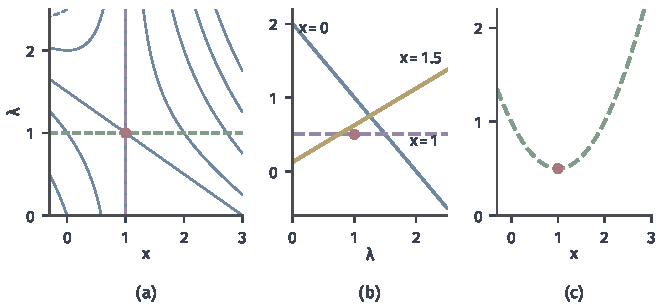
\includegraphics[width=112mm]{figures/05-optimization/06-constrained-optimization/matplotlib/dual-saddle/figure.pdf}
 \caption{一元例的Lagrange鞍点。(a)~蓝线是$\mathcal{L}(x,\lambda)=\frac12(x-2)^2+\lambda(x-1)$的等高线，红点是鞍点$(1,1)$，绿色虚线固定$\lambda=1$，紫色虚线固定$x=1$。(b)~固定$x$时$\mathcal{L}$关于$\lambda$的直线：蓝线$x=0$可行，黄线$x=1.5$不可行，紫色虚线是$x=1$。(c)~固定$\lambda=1$时关于$x$的抛物线，红点是最小点。}
 \label{fig:dual-saddle}
\end{BookInlineFigure}

\begin{theorem}[鞍点等价于两侧达到且零间隙]
 \label{thm:dual-saddle}
 $(\bm{x}^\star,\bm{\lambda}^\star,\bm{\nu}^\star)$是Lagrange鞍点，当且仅当$\bm{x}^\star$是原始最优点，$(\bm{\lambda}^\star,\bm{\nu}^\star)$是对偶最优乘子，并且式~\eqref{eq:dual-zero-gap}成立。此结论不要求问题凸。
\end{theorem}

\begin{proof}
 必要性。记鞍点处的Lagrange函数值为$\mathcal{L}^\star$。式~\eqref{eq:dual-saddle}左半边说明$\mathcal{L}(\bm{x}^\star,\cdot,\cdot)$对乘子有上界，由式~\eqref{eq:dual-sup-recovers}，$\bm{x}^\star$可行，并且上确界$f(\bm{x}^\star)\leq\mathcal{L}^\star$。

 由$\bm{\lambda}^\star\geq\bm{0}$和可行性，又有$\mathcal{L}^\star\leq f(\bm{x}^\star)$，所以
 \[
  \mathcal{L}^\star=f(\bm{x}^\star).
 \]
 式~\eqref{eq:dual-saddle}右半边说明$\bm{x}^\star$是$\mathcal{L}(\cdot,\bm{\lambda}^\star,\bm{\nu}^\star)$在$\bm{D}$上的全局最小点，所以
 \[
  q(\bm{\lambda}^\star,\bm{\nu}^\star)=\mathcal{L}^\star=f(\bm{x}^\star).
 \]
 由定理~\ref{thm:dual-zero-gap-kkt}第一部分，两侧都最优。

 充分性。设$\bm{x}^\star$可行，$\bm{\lambda}^\star\geq\bm{0}$，且式~\eqref{eq:dual-zero-gap}成立。由定理~\ref{thm:dual-zero-gap-kkt}第一部分，互补松弛成立，所以$\mathcal{L}^\star=f(\bm{x}^\star)$，且$\bm{x}^\star$全局最小化$\mathcal{L}(\cdot,\bm{\lambda}^\star,\bm{\nu}^\star)$，这是右半边。对任意$\bm{\lambda}\geq\bm{0}$和$\bm{\nu}$，由可行性，
 \[
  \mathcal{L}(\bm{x}^\star,\bm{\lambda},\bm{\nu})=f(\bm{x}^\star)+\sum_i\lambda_ig_i(\bm{x}^\star)\leq f(\bm{x}^\star)=\mathcal{L}^\star,
 \]
 这是左半边。
\end{proof}

由定理~\ref{thm:dual-saddle}，鞍点存在需要两个最优值都达到并且相等，这比强对偶强。第~\ref{sec:dual-gap-attainment}节前两个例子零间隙，却都没有鞍点，因为其中一侧没有达到。

把驻定当成鞍点是常见的错误。上一小节的$(1,2,0)$使$\nabla_x\mathcal{L}=0$，但$x=1$是$\mathcal{L}$的最大点，这组点满足KKT，却不满足式~\eqref{eq:dual-saddle}的右半边。一般的极小极大问题中交换取极值次序的条件，由第~\ref{chap:minimax-optimization}章专门研究，这里的$\mathcal{L}$对乘子是线性的，是其中结构较简单的一类。

图~\ref{fig:dual-certificate-map}和表~\ref{tab:dual-certificate-compare}把这一节的关系放在一起。中间的结论只有一个：一对候选，两边都全局最优，且目标值相等。

\begin{BookInlineFigure}
 \centering
 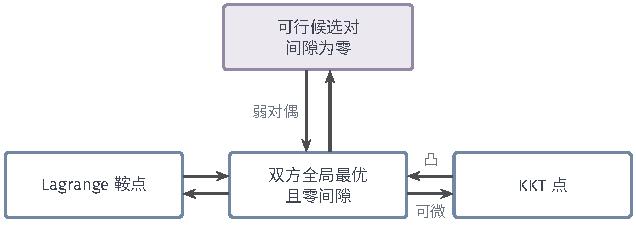
\includegraphics[width=107.8mm]{figures/05-optimization/06-constrained-optimization/tikz/dual-certificate-map/figure.pdf}
 \caption{几种最优性证据的关系。零间隙的可行候选对与“双方全局最优且零间隙”等价，后者与Lagrange鞍点等价，这三者都不要求凸性；从KKT点推出中间结论需要凸性，从中间结论推出KKT点需要在内点处可微。}
 \label{fig:dual-certificate-map}
\end{BookInlineFigure}

\begin{BookInlineTable}
 \centering
 \begin{tabular}{@{}lll@{}}
  \toprule
  证据 & 要检查什么 & 能断言什么\\
  \midrule
  KKT & 可行、符号、互补、驻定 & 凸时才全局最优\\
  候选间隙 & 可行、合法乘子、可信的$q$ & 次优性不超过间隙\\
  零间隙 & 同上，且间隙为零 & 两侧全局最优\\
  鞍点 & 式~\eqref{eq:dual-saddle}，右半为全局最小 & 与零间隙候选对等价\\
  \bottomrule
 \end{tabular}
 \caption{几种最优性证据的比较。除KKT外，其余三种证据都不要求问题凸。}
 \label{tab:dual-certificate-compare}
\end{BookInlineTable}

\section{本章小结}
\label{sec:dual-summary}

本章开头的问题是，手里有一个可行点，怎样知道它离最优还差多少。回答是对偶函数：固定一组合法乘子，对原变量在整个定义域上取下确界，得到的数就是最优值的下界。这个下界只用了下确界的定义和符号，所以弱对偶不需要凸性、可微性和约束资格。对偶函数总是凹的，但计算它的每个值都要做一次内层全局最小化。

一对候选给出的误差证书$f(\hat{\bm{x}})-q(\bm{\lambda},\bm{\nu})$有三个前提：原始可行，乘子合法，$q$算得可信。内层近似得到的值在真正的下界上方，必须扣除经过证明的误差，才能写进证书。

凸共轭把“函数加线性项取下确界”单独提取出来，二次函数、范数、约束指标函数的共轭分别对应二次项、对偶范数球和支撑函数，由此可以直接写出线性约束问题和复合问题的对偶形式。共轭能够重建适当、下半连续的凸函数，但这一点与某个具体问题的零间隙是两回事。

最好的下界是否等于最优值，取决于正则条件。Slater条件和复合问题的相对内部条件都排除了竖直的支撑超平面，保证零间隙和对偶最优乘子存在，却不保证原始最优点存在。凸性本身不能保证零间隙，零间隙也不保证两侧都达到。

实际使用时，能够核对的证据是一对候选加上间隙。零间隙的候选对同时给出两侧的全局最优性，等价于Lagrange鞍点，这些结论不要求凸性；KKT点在凸问题中才等价于它们。乘子如何解释参数的变化，由第~\ref{chap:parametric-sensitivity}章讨论；怎样在算法中实际更新乘子，由第~\ref{chap:penalty-multiplier-methods}章讨论。

